% List of figures and tables to be used
%
% 1) Clustering as a function of different bins in redshift and stellar masses
%
% 2) Weak lensing signal measurement for each of these bins (?!)
% 3) Posterior distribution of astrophysical parameters
% 4) Posterior distribution of cosmological parameters
% 5) Posterior distribution of HOD, satellite fraction, 
%
%
%
%
%
%%%%%%%%%%%%%%%%%%%%%%%%%%%%%%%%%%%%%%%%%%%%%%%%%%%%%%%%%%%%%%%%%%%%%%%%%%
% HEADER
%%%%%%%%%%%%%%%%%%%%%%%%%%%%%%%%%%%%%%%%%%%%%%%%%%%%%%%%%%%%%%%%%%%%%%%%%%

\pdfoutput=1

\documentclass[iop, apj]{emulateapj}

\usepackage{xspace}
\usepackage{amsmath}
\usepackage{framed} 
\usepackage{txfonts}
\usepackage{epstopdf} 
\usepackage{color}
\usepackage{rotating}
\usepackage{natbib}
\usepackage{ulem}
\usepackage{xspace}
\usepackage{comment}
%\usepackage{hyperref}

\newcommand{\mt}[1]{{\textcolor{blue}{#1}}}
\newcommand{\hm}[1]{{\textcolor{red}{#1}}}
\newcommand{\sm}[1]{{\textcolor{magenta}{#1}}}
\newcommand{\rachel}[1]{{\textcolor{green}{#1}}}
\newcommand{\rfix}[1]{{\textcolor{cyan}{#1}}}
\newcommand{\jcap}{JCAP}

%\hypersetup{
%  colorlinks   = true, %Colours links instead of ugly boxes
%  urlcolor     = black, %Colour for external hyperlinks
%  linkcolor    = black, %Colour of internal links
%  citecolor   = black %Colour of citations
%}

\slugcomment{To be submitted to the Astrophysical Journal}

\special{papersize=8.5in,11in}
\setlength{\pdfpageheight}{\paperheight}
\setlength{\pdfpagewidth}{\paperwidth}
\newdimen\hssize
\hssize=8.4truecm

%%%%%%%%%%%%%%%%%%%%%%%%%%%%%%%%%%%%%%%%%%%%%%%%%%%%%%%%%%%%%%%%
% Text markup
%%%%%%%%%%%%%%%%%%%%%%%%%%%%%%%%%%%%%%%%%%%%%%%%%%%%%%%%%%%%%%%%

\def\red{\color{red}}
\def\blue{\color{blue}}

%%%%%%%%%%%%%%%%%%%%%%%%%%%%%%%%%%%%%%%%%%%%%%%%%%%%%%%%%%%%%%%%
% Physical units
%%%%%%%%%%%%%%%%%%%%%%%%%%%%%%%%%%%%%%%%%%%%%%%%%%%%%%%%%%%%%%%%

\newcommand{\pc}{\>{\rm pc}}
\newcommand{\kpc}{\>{\rm kpc}}
\newcommand{\mpc}{\>{\rm Mpc}}
\newcommand{\gpc}{\>{\rm Gpc}}
\newcommand{\kpch}{\>{h^{-1}{\rm kpc}}}
\newcommand{\mpch}{\>h^{-1}{\rm {Mpc}}}
\newcommand{\gpch}{\>h^{-1}{\rm {Gpc}}}

\newcommand{\msun}{\>{\rm M_{\odot}}}
\newcommand{\lsun}{\>{\rm L_{\odot}}}
\newcommand{\msunh}{\>h^{-1}\rm M_\odot}
\newcommand{\lsunh}{\>h^{-2}\rm L_\odot}

\newcommand{\kmsmpc}{\>{\rm km}\,{\rm s}^{-1}\,{\rm Mpc}^{-1}}
\newcommand{\kms}{\>{\rm km}\,{\rm s}^{-1}}
\newcommand{\cm}{\>{\rm cm}}

\newcommand{\erg}{\>{\rm erg}}
\newcommand{\yr}{\>{\rm yr}}
\newcommand{\yrs}{\>{\rm yrs}}
\newcommand{\kdegree}{\>{\rm K}}
\newcommand{\kev}{\>{\rm keV}}

%%%%%%%%%%%%%%%%%%%%%%%%%%%%%%%%%%%%%%%%%%%%%%%%%%%%%%%%%%%%%%%%
% Physical quantities & variables
%%%%%%%%%%%%%%%%%%%%%%%%%%%%%%%%%%%%%%%%%%%%%%%%%%%%%%%%%%%%%%%%

\def\LCDM{$\Lambda$CDM\ }

\def\mvir{M_{\rm vir}}
\def\rvir{R_{\rm vir}}
\def\gcm3{\mathrm{g} / \mathrm{cm}^3}

\newcommand{\mbh}{M_{\bullet}}
\newcommand{\vrot}{V_{\rm rot}}
\newcommand{\tvir}{T_{\rm vir}}
\newcommand{\vesc}{V_{\rm esc}}

%%%%%%%%%%%%%%%%%%%%%%%%%%%%%%%%%%%%%%%%%%%%%%%%%%%%%%%%%%%%%%%%
% Statistics and maths
%%%%%%%%%%%%%%%%%%%%%%%%%%%%%%%%%%%%%%%%%%%%%%%%%%%%%%%%%%%%%%%%

\def\chidof{\chi^2/N_{\rm dof}}

%%%%%%%%%%%%%%%%%%%%%%%%%%%%%%%%%%%%%%%%%%%%%%%%%%%%%%%%%%%%%%%%
% General equations, greater than etc.
%%%%%%%%%%%%%%%%%%%%%%%%%%%%%%%%%%%%%%%%%%%%%%%%%%%%%%%%%%%%%%%%

\def\gtsima{$\; \buildrel > \over \sim \;$}
\def\ltsima{$\; \buildrel < \over \sim \;$}
\def\prosima{$\; \buildrel \propto \over \sim \;$}
\def\gsim{\lower.7ex\hbox{\gtsima}}
\def\lsim{\lower.7ex\hbox{\ltsima}}
\def\simgt{\lower.7ex\hbox{\gtsima}}
\def\simlt{\lower.7ex\hbox{\ltsima}}
\def\simpr{\lower.7ex\hbox{\prosima}}

\newcommand{\avg}[1]{\langle #1 \rangle}

\newcommand{\degree}{\ensuremath{^\circ}}

%%%%%%%%%%%%%%%%%%%%%%%%%%%%%%%%%%%%%%%%%%%%%%%%%%%%%%%%%%%%%%%%
% Non-italic letters
%%%%%%%%%%%%%%%%%%%%%%%%%%%%%%%%%%%%%%%%%%%%%%%%%%%%%%%%%%%%%%%%

\def\rma{{\rm a}}
\def\rmb{{\rm b}}
\def\rmc{{\rm c}}
\def\rmd{{\rm d}}
\def\rme{{\rm e}}
\def\rmf{{\rm f}}
\def\rmg{{\rm g}}
\def\rmh{{\rm h}}
\def\rmi{{\rm i}}
\def\rmj{{\rm j}}
\def\rmk{{\rm k}}
\def\rml{{\rm l}}
\def\rmm{{\rm m}}
\def\rmn{{\rm n}}
\def\rmo{{\rm o}}
\def\rmp{{\rm p}}
\def\rmq{{\rm q}}
\def\rmr{{\rm r}}
\def\rms{{\rm s}}
\def\rmt{{\rm t}}
\def\rmu{{\rm u}}
\def\rmv{{\rm v}}
\def\rmw{{\rm w}}
\def\rmx{{\rm x}}
\def\rmy{{\rm y}}
\def\rmz{{\rm z}}

\def\rmA{{\rm A}}
\def\rmB{{\rm B}}
\def\rmC{{\rm C}}
\def\rmD{{\rm D}}
\def\rmE{{\rm E}}
\def\rmF{{\rm F}}
\def\rmG{{\rm G}}
\def\rmH{{\rm H}}
\def\rmI{{\rm I}}
\def\rmJ{{\rm J}}
\def\rmK{{\rm K}}
\def\rmL{{\rm L}}
\def\rmM{{\rm M}}
\def\rmN{{\rm N}}
\def\rmO{{\rm O}}
\def\rmP{{\rm P}}
\def\rmQ{{\rm Q}}
\def\rmR{{\rm R}}
\def\rmS{{\rm S}}
\def\rmT{{\rm T}}
\def\rmU{{\rm U}}
\def\rmV{{\rm V}}
\def\rmW{{\rm W}}
\def\rmX{{\rm X}}
\def\rmY{{\rm Y}}
\def\rmZ{{\rm Z}}

\def\calA{{\cal A}}
\def\calB{{\cal B}}
\def\calC{{\cal C}}
\def\calD{{\cal D}}
\def\calE{{\cal E}}
\def\calF{{\cal F}}
\def\calG{{\cal G}}
\def\calH{{\cal H}}
\def\calI{{\cal I}}
\def\calJ{{\cal J}}
\def\calK{{\cal K}}
\def\calL{{\cal L}}
\def\calM{{\cal M}}
\def\calN{{\cal N}}
\def\calO{{\cal O}}
\def\calP{{\cal P}}
\def\calQ{{\cal Q}}
\def\calR{{\cal R}}
\def\calS{{\cal S}}
\def\calT{{\cal T}}
\def\calU{{\cal U}}
\def\calV{{\cal V}}
\def\calW{{\cal W}}
\def\calX{{\cal X}}
\def\calY{{\cal Y}}
\def\calZ{{\cal Z}}

\def\ba{{\bf a}}
\def\bb{{\bf b}}
\def\bc{{\bf c}}
\def\bd{{\bf d}}
\def\be{{\bf e}}
\def\bff{{\bf f}}
\def\bg{{\bf g}}
\def\bh{{\bf h}}
\def\bi{{\bf i}}
\def\bj{{\bf j}}
\def\bk{{\bf k}}
\def\bl{{\bf l}}
\def\bm{{\bf m}}
\def\bn{{\bf n}}
\def\bo{{\bf o}}
\def\bp{{\bf p}}
\def\bq{{\bf q}}
\def\br{{\bf r}}
\def\bs{{\bf s}}
\def\bt{{\bf t}}
\def\bu{{\bf u}}
\def\bv{{\bf v}}
\def\bw{{\bf w}}
\def\bx{{\bf x}}
\def\by{{\bf y}}
\def\bz{{\bf z}}

\def\bA{{\bf A}}
\def\bB{{\bf B}}
\def\bC{{\bf C}}
\def\bD{{\bf D}}
\def\bE{{\bf E}}
\def\bF{{\bf F}}
\def\bG{{\bf G}}
\def\bH{{\bf H}}
\def\bI{{\bf I}}
\def\bJ{{\bf J}}
\def\bK{{\bf K}}
\def\bL{{\bf L}}
\def\bM{{\bf M}}
\def\bN{{\bf N}}
\def\bO{{\bf O}}
\def\bP{{\bf P}}
\def\bQ{{\bf Q}}
\def\bR{{\bf R}}
\def\bS{{\bf S}}
\def\bT{{\bf T}}
\def\bU{{\bf U}}
\def\bV{{\bf V}}
\def\bW{{\bf W}}
\def\bX{{\bf X}}
\def\bY{{\bf Y}}
\def\bZ{{\bf Z}}
% Frequently used expressions

\def\ms{$M-\sigma$\xspace}
\def\msr{$M-\sigma$ relation\xspace}

\def\sigr{\sigma(R)}
%\def\sigsr{\sigma(<R)}
\def\sgmr{\sigma / \sqrt{G M(R) / R}}
\def\sp{\sigma'}

\def\rdelta{R_{\Delta}}
\def\mdelta{M_{\Delta}}
\def\rs{r_{\rm s}}
%\def\rc{r_{\rm c}}

\def\mr{$M/R$\xspace}
\def\fpe{f_{\rm PE}}

\def\rhot{\rho_{\Delta}}
\def\rhotm{\rhot^{1/2} M}
\def\rhotmz{\rhot(z)^{1/2} M(z)}
\def\rhoc{\rho_{\rm c}}
\def\rhom{\rho_{\rm m}}

% Mass definitions. We cannot define macros with numbers in them

\def\cvir{c_{\rm vir}}

\def\mtom{M_{\rm 200m}}
\def\rtom{R_{\rm 200m}}
\def\ctom{c_{\rm 200m}}

\def\msfm{M_{\rm 740m}}
\def\rsfm{R_{\rm 740m}}
\def\csfm{c_{\rm 740m}}

\def\mtoc{M_{\rm 200c}}
\def\rtoc{R_{\rm 200c}}
\def\ctoc{c_{\rm 200c}}

\def\mfoc{M_{\rm 500c}}
\def\rfoc{R_{\rm 500c}}
\def\cfoc{c_{\rm 500c}}

\def\mtfc{M_{\rm 2500c}}
\def\rtfc{R_{\rm 2500c}}
\def\ctfc{c_{\rm 2500c}}

\def\rone{{\bf r_1}}
\def\rtwo{{\bf r_2}}
\def\rhalo{{\bf r_\rmh}}

\newcommand{\?}{\stackrel{?}{=}}

\shorttitle{Stacked cluster lensing profile with NFW scaling}
\shortauthors{Niikura et al.}

\begin{document}

%%%%%%%%%%%%%%%%%%%%%%%%%%%%%%%%%%%%%%%%%%%%%%%%%%%%%%%%%%%%%%%%%%%%%%%%%%
% EPS OR PDF FIGURES
%%%%%%%%%%%%%%%%%%%%%%%%%%%%%%%%%%%%%%%%%%%%%%%%%%%%%%%%%%%%%%%%%%%%%%%%%%
%
\def\figdir{.}
\def\figext{pdf}

%%%%%%%%%%%%%%%%%%%%%%%%%%%%%%%%%%%%%%%%%%%%%%%%%%%%%%%%%%%%%%%%%%%%%%%%%%
% TITLE ETC
%%%%%%%%%%%%%%%%%%%%%%%%%%%%%%%%%%%%%%%%%%%%%%%%%%%%%%%%%%%%%%%%%%%%%%%%%%

\title{Detection of universality of dark matter profile from Subaru 
weak lensing measurements of 50 massive clusters}
\author{Hiroko~Niikura\altaffilmark{1,2},
Masahiro~Takada\altaffilmark{1},
....
}

\affil{
$^1$ Kavli Institute for the Physics and Mathematics of the Universe
(WPI), TODIAS,
%Todai Institutes for Advanced Study,
The
University of Tokyo, 
%5-1-5 Kashiwanoha, Kashiwa-shi, 
Chiba, 277-8583, Japan \\
$^2$ Physics Department, The University of Tokyo, Bunkyo, Tokyo
113-0031, Japan
}
\begin{abstract}
TBD
\begin{comment}
We present new limits of the dark matter halo..
By fully taking advantage of the wide field-of-view of Hyper Suprime-Cam, which allows us to cover the entire bulge and disk regions of Andromeda Galaxy (M31) 
with one point, we use the dense cadence data of M31 (about 190 images of 90sec 
exposure  each over about 7 hours) in order to search for microlensing events 
of stars in M31 due to foreground primordial black holes (PBH).  
PBH is one of viable candidates of dark matter, and might dominate the dark 
matter in both the halo regions of Milky Way and M31. We aim at constraining 
the abundance of PBHs of mass scales, $10^{-9}$-$10^{-7}M_\odot$, with the 
dense-cadence HSC data. However, the PBH search requires an exquisite data 
reduction technique, especially image difference technique in such a dense star 
region needed to find transient objects (stars). We have extensively used the 
HSC pipeline to make the data reduction and here report the current status of 
this project (the results of other transients and the PBH microlensing search).
\end{comment} 
\end{abstract}

\section{Introduction}
%\citep{Okabeetal:10,Okabeetal:13}
%TBD
%PBH introduction 
The properties of dark matter has been studied from many aspects with 
observations and simulations. The previous studies have suggested that dark 
matter is non-baryonic, non-relativistic, and interacts with ordinary matter 
only via gravity. Currently unknown stable particle(s) beyond the Standard 
Model of Particle Physics is considered as viable candidates, so-called Weakly 
Interacting Massive Particles (WIMPs). However they haven't been yet detected 
neither in elastic scattering experiment nor by collider experiments. 
Primordial black hole is another viable candidate of dark matter, which was 
first proposed by \citet{Hawking:74}. A scenario of PBH dark matter does not 
require new stable particles. The mass range of PBH varies depending on the 
formation scenario in the early universe \citep{Carretal:10}. 


\section{Gravitational Microlensing of Hyper Suprime-Cam Data-3}

%{\it Explain the sample of 50 clusters}
%We make use of the same weak leasing shear catalogue with Okabe et al.(2013).
%\begin{itemize}
%\item introduction of MACHO microlensing
Gravitational microlensing effect is a unique way to probe dark matter candidate, first proposed by Paczy${\rm \acute{n}}$ski (1986). In microlensing regime, the flux of background star is magnified by the gravitational field of foreground object when they come in line of sight. Thus dark components can be detected through the magnification of background stars while they move. 
Previous microlensing studies using data such as OGLE and MACHO projects have already succeeded to detect MACHOs. The current upper limits on an abundance of PBH covers almost full range of mass scales we are interested in \citep{Capelaetal:13b}. Nevertheless, it is worth further exploring a more stringent limit on the PBH abundance. 

%\item Hyper Suprime-Cam and advantage for microlensing
In this study we propose a transient search for M31 dense-star region, using Hyper Suprime-Cam at Subaru telescope. Hyper Suprime-Cam (HSC) is a wide-field imaging camera attached at the prime focus of Subaru telescope. This camera consists of $116$ CCD chips; $104$ for science, $4$ for auto-guide, and $8$ for auto-focus,  and each CCD has 2k x 4k pixels, with a pixel scale of $0.168$ arcsec. One unique characteristic of this camera is the wide field of view (FoV) as large as $1.5$ degree at a single frame, which is three times larger than the size of full Moon in radius. Also high resolution is expected owing to the large primary mirror of 8.2 meters in effective diameter and low humidity of the summit of Mauna Kea. 261 robotic fingers keep the primary mirror in a perfect shape no matter where the telescope is pointing in the sky. 
%The filter transmittance is shown by Fig.~\ref{fig:filter} using the HSC filter model\footnote{http://subarutelescope.org/Observing/Instruments/HSC/sensitivity.html} including quantum efficiency of fully depleted CCDs (FDCCDs), transmittance of the dewar window, transmittance of the Primary Focus Unit of the HSC (POpt2), and reflectivity of the Primary Mirror. 
%
%\begin{figure}[t]
%\centering
%\includegraphics[width=10cm,clip]{pic/filter_hsc.pdf}
%\caption{\small{{
%The total transmission curve for each broad-band filter of the Subaru/Hyper Suprime-Cam system. Each curve takes into accounts the transmission of each filter, quantum efficiency of fully depleted CCDs, transmittance of the dewar window, transmittance of the Primary Focus Unit of the HSC (POpt2), and reflectivity of the Primary Mirror. }}}
%\label{fig:filter}
%\end{figure}

%We expect a large number of transient candidates in the dense star region of M31. 
The M31 is the largest spiral galaxy in the neighbor of Milky Way and is about $770$kpc away from us. 
%Comparison with Kepler...?
Our survey expects higher event rate of PBH microlensing than the previous search, owing to the wide field-of-view and excellent image quality for the dense star field. The one pointing of HSC can cover the entire bulge and disk regions of M31. However, the analysis is expect to be not straightforward; for example, reduction procedures need some careful treatments because no previous transient search performed a careful reduction for images with such a dense field taken by highly resolved wide field camera. 
%Also many stars, especially in bulge and disky regions of the M31, can be in one CCD pixel; that is, each star cannot be resolved even by the HSC/Subaru. 
Thus we will develop the method to optimize the transient analysis using the software called HSC-pipe. 




%\item 
%Mention about target mass range..?
%\end{itemize}

\section{Formulas-2}
\label{sec:pointlens}
microlensing and analytic estimate, numerical estimate, including event rate?
\subsection{Point-Source Microlensing}
General relativity predicts that a background object can be significantly brightened by strong lensing if the background and foreground objects are almost perfectly aligned along the line of sight of an observer. We can use the lensing magnification to search for an invisible, small compact object that is a possible candidate of dark matter and, if so, should exist in the halo regions of the Milky Way and M31 Galaxy. 

Here we describe the observational properties of lensing magnification. Note that we assume that source star is a star in M31, and we don't consider that a star in the MW halo region is a source star in our analysis. 
%, as illustrated in Fig.~\ref{fig:mlscheme}. 
We denote, by $\beta$, the angle between the lens and the source object on the sky, and 
$\alpha$ as the angular separation between the source and the image.
We also define the following distances; 
$r_0$ as the distance between the lens and the image in the lens plane,
$r$ between the lens and the image, 
$D_S$ as the distance between the observer and the source, and 
$x$ as the distance to the lens normalized by $D_S$. 
Then $\beta$ and $\alpha$ can be described as:
$\beta={r_0}/{x{D_S}}$, and $\alpha={r}/{x{D_S}}$. 

The total magnification of the lensed image is given by 
% 
\begin{eqnarray}
A=A_{1}+A_{2}=\frac{u^2+2}{u\sqrt{u^2+4}}, \quad u\equiv\frac{r_0}{R_E}
\label{eq:cano}
\end{eqnarray}
%
%
where $R_E$ is Einstein radius defined as:  %
\begin{eqnarray}
R^2_E=\frac{4GMD}{c^2},\quad D\equiv D_S x(1-x)
\end{eqnarray}
%
The magnification of source image varies with time as the lens object moves in front of the source object. Here we define $v$ as the relative velocity component of the lens object perpendicular to the line of sight, and $d$ as the closest distance of lens to the line of sight. The closest distance to the lens image can also be characterized by the impact parameter, defined as $u_{\rm min}={d}/{R_S}$. 
Here we define a typical time scale of the magnification time variation as $t_0={R_E}/{v}$. 
By characterizing the time variation of lens flux with this parameter, we obtain 
%
%\begin{eqnarray}
%\left(v(t-t_{\rm max})\right)^2+d^2=r^2_0
%\label{eq:mmtimescale}
%\end{eqnarray}
%
%
\begin{eqnarray}
u^2=\frac{r^2_0}{R^2_E}=\frac{(t-t_{\rm max})^2}{t^2_0}+u^2_{\rm min}
\label{eq:cimpa}
\end{eqnarray}
%
where $t_{\rm max}$ is the time when the lens and the source are in the closest separation on the sky. 
%Hence the flux magnification of microlensing event is given by a function of time as:
%
%\begin{eqnarray}
%A(t)=\frac{y^2+u^2_{\rm min}+2}{\sqrt{y^2+u^2_{\rm min}}\sqrt{y^2+u^2_{\rm min}+4}},\quad y=\frac{t-t_{\rm max}}{t_0}, 
%\end{eqnarray}
%
%which implies that magnification is larger for smaller impact parameter $u_\mathrm{min}$. Note that neither the wavelength of the light ray observed nor the original luminosity of the source alter an amount of the lensing magnification. 
%
%\begin{figure}[t]
%\centering
%\includegraphics[width=13cm,clip]{pic/microlensing_Bohdan.pdf}
%\caption{\small{Simulated light curves for microlensing events, taken from Fig. 2 of Paczy${\rm \acute{n}}$ski (1986). Each light curve stands for different impact parameter $u_\mathrm{min}$ at 0.1, 0.2, ..., 1.1, 1.2, and light curve with larger magnification amplitude corresponds to smaller $u_\mathrm{min}$ parameter. }}
%\end{figure}
%
If a source star is located at $D_S=770$ {kpc}, the standard timescale of microlensing event  $t_0={R_E}/{v}$ %as in Eq.~(\ref{eq:mtimescale}) 
is given by: 
%
\begin{eqnarray}
t_0\simeq1.8{\rm hours} \left(\frac{M}{10^{-7}M_\odot}\right)^{\frac{1}{2}}\left(\frac{xD_S}{100 \rm{kpc}}\right)^{\frac{1}{2}} \left(\frac{200 {\rm km/sec}}{v}\right)
\end{eqnarray}
%
where we assumed that a target mass of PBH is $10^{-7}M_\odot$, $D_L=100$kpc for a distance to the lens PBH, and $V_\mathrm{halo}=200$km/sec for the perpendicular velocity component of the lens. 


\subsection{Finite-Source Microlensing-2}
\subsection{Finite-Source Microlensing with Limb-Darkening-2}
\subsection{Effect of Limb Darkening on the Numerical Estimate of Expected Number of Events-2(new sec.)}

\subsection{Light curve characterization in pixel lensing regime}
The property of microlensing event is characterized by two factors: magnification amplitude and event duration. These two quantities are characterized by the Einstein time scale $t_E$ and the maximum magnification of the light curve, $A_0$.
As we described, our definition of microlensing is the case that a source star enters within the Einstein radius of PBH, which correspond to the magnification $A>1.34$. In the pixel lensing method we need to discriminate the lensed star from other stars. 
When extracting the physical parameters from the observed light curve of microlensing, it is known that the fitting gives a strong degeneracy between the Einstein time scale ($t_E$) and the impact parameter $\beta$ \citep{Gould:96,BaltzSilk:00}. 

In order to quantify the microlensing event, we adopt two observables for characterizing the events following \citet{Riffeseretal:06}: the full-width-half-maximum timescale of the event ($t_\mathrm{FWHM}$) and the flux excess above the background ($\Delta F$). These two quantities are related to the canonical microlensing parameters as following: 
%
First we characterize the event duration as the full width of the half-maximun peak in the light curve. 
By definition, $t_\mathrm{FWHM}$ of a light curve can be described as: 
%
\begin{eqnarray}
A\left(\frac{t_{\rm FWHM}}{2}\right)-1\equiv\frac{A_0-1}{2}
\end{eqnarray}
%
where $A_0$ represents the maximum magnification of the light curve. Here we will characterize the timescale as a function of impact parameter $\beta$, the quantity described as $u_\mathrm{min}$ in Eq.~(\ref{eq:cimpa}). Then we can rewrite the timescale in the same way as described in \citet{Gondolo:99}: 
%
\begin{eqnarray}
t_{\rm FWHM}=t_{\rm E}\omega(\beta)
\end{eqnarray}
%
where 
%
\begin{eqnarray}
\omega(\beta)=2\sqrt{2f(f(\beta^2))-\beta^2},
\end{eqnarray}
%
\begin{eqnarray}
f(x)=\frac{x+2}{\sqrt{x(x+4)}}-1
\end{eqnarray}
%
where $\omega(\beta)$ satisfies $\omega(\beta\ll1)\simeq \beta\sqrt{3}$, and $\omega(\beta\gg1)\simeq\beta(\sqrt{2}-1)^{0.5}$. 
Next we describe another parameter to represent the amplitude of light curve. In image difference technique it is much convenient to adopt the maximum flux of the event instead of maximum magnification: 
%
\begin{eqnarray}
\Delta F_{\rm max}=F_0\left(\frac{\beta^2+2}{\beta\sqrt{\beta^2+4}}-1\right)
\label{eq:diffmicro}
\end{eqnarray}
%
where $\Delta F$ represents the excess flux due to microlensing effect. Following the image difference technique we can set the detection threshold flux $\Delta F_{\rm det}$ as: 
$\Delta F_{\rm det}\equiv F(t)-F_{\rm ref}=\Delta F_{\rm bl}+F_0(A(t)-1)$. 
Note that $\Delta F_{\rm bl}=0$ holds for case where the source is not affected by gravitational lensing effect. 




\section{Data Analysis and Event Selection-3}
\label{sec:obs2}
%observations and photometric reductions

\subsection{Observation}
\label{sec:obsm31}
%\begin{itemize}
%\item[(1)]{\bf Methodology of transient survey : pixel lensing}\\
A search of microlensing events requires a precise photometry of stars. 
The HSC pointing of our observation was determined so as to cover the entire region of M31, from the inner bulge to the outer disk regions, with its one pointing. Hence the pointing is centered at the coordinates of the M31 central region: (RA, dec) = (00h 42m 44.420s/+41d 16m 10.1s). 
As we described above, we need to compare/differentiate the total flux of the same CCD pixel between different exposures in order to find transient candidates. That is, we want to measure the same (multiple) stars by the same CCD pixel, because we then care only about the relative flux difference in the same pixel of different exposures (do not care about an absolute flux calibration between different pixels). Therefore, we did not employ any dithering strategy for our observation. However, in reality the HSC/Subaru system has an imperfect accuracy of auto-guiding and/or pointing, so we have found  variations in the pointings of different exposures, by a few pixels up to pixels, as we will discuss later. 

Our observation was conducted in November 23, 2014 on dark night, one day after new moon. We acquired the 194 exposures of M31 for about 7 hours starting from sunset of the day until the elevation of M31 on the sky becomes down to about $30$  degrees. The sampling rate of images is about $2$ minutes, $90$ seconds for each exposure and about $30$ seconds for readout.All images were taken in $r$-band filter, corresponding to $0.64$ $\mu$m in wavelength. The visibility (elevation) of M31 and the seeing size of each exposure are given in Fig.~\ref{fig:seeing}. Here the ``seeing'' is a commonly-used quantity to characterize a spatial resolution of an image, i.e. the size of the point spread function (PSF) of the image. 
%
%\begin{figure}[t]
%\centering
%\includegraphics[width=8cm,clip]{pic/m31_visibility.pdf}
%\includegraphics[width=8cm,clip]{pic/seeing.pdf}
%\caption{\small{Characteristics of our HSC M31 observation. {Left panel} shows the time-variation of altitude of target field (M31) during observation. Our observation started from 18:33:59 on November 24 2014, and ended at 1:35:34 when the altitude gets lower than $30$ degrees. {Right panel} shows the seeing of each exposure. We conducted the ``focusing'' (determined the focus position of the camera) three times during the night, 19:50:33, 22:37:02, and 0:37:07. }} 
%\label{fig:seeing}
%\end{figure}
%
%\end{itemize}

In the previous microlensing study in Large Magellanic Cloud (LMC), another dense-star region, the photometry on each star is achieved because of its proximity; only $50$ kpc away from us \citep{Alocketal:00}. However, this is not the case for M31. As M31 is about $770$ kpc away and further than LMC, multiple stars can be in the same CCD pixel. 
In order to measure the time variation of flux in such a crowded imaging data, we adopt a method called pixel lensing \citep{AlardLupton:98}. Even when multiple stars locate in a pixel, we can trace the change of flux in a pixel unit. Thus we can extract the location of variable candidates assuming that there is only one variable star in a pixel. In addition we adopt a technique so-called image difference to make comparison between images in different time frames. 
Image difference technique is also helpful for precise photometry in pixel lensing regime because we can cancel the effect from surrounding stars (see Sec~\ref{sec:obstrans} for the detail). As this comparison requires an accurate astrometry matching between different frames, we use the reference image generated by combining best-seeing frames to perform the image difference between the reference image and a target frame image in order to minimize effects of imperfect astrometry. 


\subsection{Data reduction}
\label{sec:obsreduce}
\label{sec:obstrans}
The data itself contains only flux information (more exactly, ADU counts) in pixel coordinate. 
A precise photometry requires a correction of various systematic effects such as night glow, instrument noise, vignetting of the camera, and variations in responses between different CCD pixels.  

%We have used the . 
%We have developed 
All data reduction was done using the HSC pipeline, the specialized software package that has been developed for the HSC SSP program, being led by scientists at Kavli IPMU, Princeton University and NAOJ. 

After the above basic data processing, we need to subtract background contamination due to light diffusion of the atmosphere or other unknown source -- background subtraction. However, the background subtraction for the M31 region is quite challenging, because there is no blank region and every CCD chip is to some extent affected by unresolved, diffuse stellar light. Hence, we would suffer from an an under- or over-subtraction. Nevertheless, since we are mainly interested in time-variable stars, we tried to perform the two methods of background subtraction, as will be described in \S~\ref{sec:back6d} in detail. 

We further need to correct for effects of cosmic rays. For the fully-depleted CCDs, cosmic ray events imprint a characteristic trail-like image. For a blank field, it is relatively straightforward to identify the CR image from the trail-like image, or by combining several exposures. However, the CR removal is not so straightforward for the dense star field we are working on. We skipped the CR removal for simplicity, and will discuss the residual effect later. 


To implement the difference image technique in order to find transient candidates, we used the following methods:
%\item
%{WCS determination}\\
Here we describe how to determine the WCS coordinate system for 194 exposures. In addition to our fiducial exposures each of which is a 90 sec exposure data, we also took 30 sec exposure at the beginning of our observation, because bright stars are less saturated in the short exposure, and therefore we can use more stars for astrometry determination. By using the star catalog of Pan-Starrs survey as the input catalog for the M31 region, we solved astrometry solution of every 11 images, 30 sec exposure plus time-sequential 10 exposures taken from the science 194 exposures. 

The HSC pipeline provide us with a useful feature, the so-called ``SkyMap'', which defines a conversion of the celestial sphere to the flat coordinate system, ``SkyMap coordinate'', based on a tiling or tessellation. The largest region in the coordinate  is called a ``Tract'', and it contains a ``Patch''. These processes performed a warping of each exposure to determine the common WCS of the SkyMap.
%
%\begin{figure}[t]
%\centering
%\includegraphics[width=6.5cm,clip]{pic/m31_r_image_quick.pdf}
%\includegraphics[width=8cm,clip]{pic/m31_r_image.pdf}
%\caption{\small{An example of our exposure image of the M31 region. {Left panel} displays one raw image taken by Hyper Suprime-Cam. Each rectangle-shape sub region, enclosed by black-color gap, corresponds to a single CCD chip. {Right panel} shows one example of reduced image, the one later called as reference image in z-scale (The detail of this image is described in \S~\ref{sec:refimage}). This figure is in a unit called ``tract'',  composed of sub-regions called ``patches'' (displayed as different-color rectangular regions in this figure). }}
%\label{fig:patch}
%\end{figure}
%

After the basic data reduction as mentioned in the previous section, we apply the image difference technique to the 194 exposures in order to search for transient candidates. 
%In the following, we describe procedures that we used for our transient search. 


\subsection{Selection criteria of variable candidates}
\label{sec:detecmethod}
\subsubsection{Identification of variable objects}
Making the image difference or image subtraction comparing different exposures is one of the most important data processes for our science. If two exposures to be compared have same seeing, same pointing and similar sky noise, the image difference would be straightforward. However, our 194 exposures have quite different seeing sizes (ranging from $0.4''$ to $1.6''$), and have variations in the pointing accuracy (within 5 pixels between time-sequential two exposures). In addition, the M31 field contains dense, crowded star regions. Hence, we need to make a more careful analysis. 

To have a robust result of the image difference, we combined or coadded 10 best-seeing size exposures among the 194 exposures to generate the ``reference'' image, where the 10 exposures are not time sequential (but most of the 10 exposures are from the data in 3 hours from the observation start). 
Fig.~\ref{fig:seeing} shows how the seeing size changes with time from the observation start. For a target image to be compared with the reference image, we coadded the 5 time-sequential exposures to generate the target image with improved signal-to-noise ratio. We have 37 target images (note that the target images might contain some exposures used in the reference image). Hence, we have $37$ time-sequential target images, given in the units of SkyMap patches. Our method thus has a sensitivity to find transient objects with time scales longer than 10min. 

We subtract the reference image from each of the 37 target images in order to generate the difference image. 
Fig.~\ref{fig:diffeg} shows an example of the difference image. 
Almost all the stars are cleanly subtracted. Note that, if a single visit is used to compare with the reference image, cosmic rays show up in the difference image. This is another region to use the coadd image of 5 exposures for the image difference. We expect that an object that has a flux change shows up in the difference image (for this particular example, there is no secure candidate of variable star). 
Note that there are several failure regions in performing the image subtraction. For example, in the bulge region of M31, we cannot construct the coadd images because there are too many stars and we cannot solve the astrometry from the distribution of identified stars.  
%The summary of image difference scheme is given in Fig.~\ref{fig:detectionsche}. 
%flow chart should be here!

%detection threshold
As we described, we constructed the 37 difference images by comparing each of 37 time-sequential coadded images with the reference image. Since time separation between the 37 coadded images is about 10min, we can search for transient candidates whose variations are longer than 10 minutes. Our main interest is variable stars, and we need to exclude fake candidates arising from cosmic rays, fakes due to imperfect image subtraction (e.g. around bright stars), and so on. 

To remove obvious fakes in the first step, we impose the following conditions to identify transient candidates, based on the fact that the secure candidates should look like a PSF image in the difference image. 
%
\begin{itemize}
\item{minSizeRatio (Mininum value of size ratio of detected source and PSF): $0.75$}
\item{maxSizeRatio (Maximum value of size ratio of detected source and PSF): $1.25$}
\item{limAxisRatio (Limit value to be consistent with PSF): $0.75$}
\item{maxResidual (Maximum value of residual after PSF subtraction): $3.0$}
\item{thresholdValue (Threshold of signal to noise ratio of PSF counts): $5.0$}
\end{itemize}
%
The former two conditions exclude candidates which looks unlikely to be a point source; {\it minSizeRatio} excludes candidates whose shapes are very elongated, and {\it maxSizeRatio} mainly excludes those with tiny, vague shapes. The latter two conditions are imposed concerning the flux distribution. As mentioned before, variable star candidates are expected to have a point-source flux distribution that can be therefore well fitted by the PSF in the image. Thus {\it limAxisRatio} condition excludes candidates whose flux distribution cannot be well fitted by PSF in the difference image. In addition {\it maxResidual} removes candidates whose residual image after subtraction of the fitted PSF image is too large. Finally {\it thresholdValue} selects candidates whose PSF magnitude in the difference image satisfies S/N$>5$. 

We identify secure candidates that pass all the above conditions. However, the number of identified transient candidates in the 37 difference images are still too many, although the images with worse seeing size tend to give us a smaller number of the candidates. 
Fig.~\ref{fig:unlikes} shows typical fake candidates that passed the above conditions. In particular, the number of survived fakes changes a lot depending on a chosen threshold value of {\it limAxisRatio}. However, we consider the upper conditions are loose enough to pick up any real variable candidate because they already pick up many fake events. One important note is that median subtraction around a target greatly helps to reduce some fakes (see the detail in \S~\ref{sec:detmedisub}). 

After the detection selections we construct a catalog of variable candidates, 
simply grouping those within ${\pm 2}$ pixels in pixel coordinates from the $37$ different-time frames.  %The properties of variable candidates is described in detail on \S~\ref{sec:candidates}. 


\subsubsection{photometry}
\label{sec:photometh}
Once a secure candidate of time-variable point source is found, we have to make a photometry of the candidate in order to measure the light curve. However, the photometry in a dense star region, where multiple stars exist in each CCD pixel, is difficult. To overcome this difficulty, we use the following method by making best use of the difference image. 
For a secure candidate found based on the above method, we first determine the WCS position of the candidate in the difference image. Then we measure the PSF magnitude at the WCS position of the candidate in the reference image that is deepest and has the highest spatial resolution: 
%
\begin{eqnarray}
m_{\rm Ref}=-2.5\log\left(\frac{C_\mathrm{Ref}}{\rm{fluxmag}0_{\rm Ref}}\right)
\end{eqnarray}
%
where $C_\mathrm{Ref}$ is the counts of the PSF photometry and $\rm{fluxmag}0_{\rm Ref}$ is the magnitude zero point of the reference image. Then we also perform the PSF photometry at the same WCS position of the candidate in the {\it  difference image} of each target exposure, rather than in the original image. In this way we believe that we can measure the change in the PSF flux for the candidate. By adding the PSF magnitude to the magnitude in the reference image, we can estimate the apparent magnitude of the candidate in the target image:
%
\begin{eqnarray}
m_{\rm i}=-2.5\log\left(\frac{C_\mathrm{i,diff}+C^{\rm i,diff}_{\rm Ref}}{\rm{fluxmag}0_{\rm i,diff}}\right)
\end{eqnarray}
%
where $C_\mathrm{i,diff}$ is the counts of the candidate for the i-th target image. 
%


\subsubsection{Impacts of different data processing methods}
\label{sec:methtest}
As we stressed several times, a photometry in a dense star region of M31 is very challenging. Hence, the different data processing methods change the photometry results of time-variable point-source candidates. Here we discuss effects of different analysis methods. 

\begin{itemize}
\item[(1)]{\it Background subtraction for single-frame processing}\\
\label{sec:back6d}
As we stressed in \S~\ref{sec:obstrans}, 
background subtraction is an important process for precise photometry (see \S~\ref{sec:obstrans} for the detail). 
This process, however, is not simple especially for a wide field imaging data like HSC. Normally we divide each CCD chip into different meshes (the default subdivision is done into 64 meshes in each CCD chip), and then estimate a smooth background by spline-interpolating the average counts over different meshes. However, the spline fitting does not work well because a large number of stars in each CCD chip cause a large variation of background counts even within the chip. Thus a over- or under-subtraction of the background counts can often happen, leaving an inhomogeneous pattern in the background-subtracted image. %as shown in the right panel of Fig.~\ref{fig:inhomo}.  
In order to overcome this inaccuracy, we employed a higher-order polynomial fitting of the background. We employed the 10-th order polynomial fitting for the CCD chips around the bulge region, which are particularly dense star regions. For other CCD chips, we used the 6-order polynomial fitting. 

%
The different background subtraction methods lead to a different number of time-variable candidates. 
Fig.~\ref{fig:m31fit} compares the distributions of identified candidates based on the different subtraction methods, the spline-fitting method (right panel: the default method of HSC pipeline) and the polynomial fitting method developed in this paper (left panel). 
The number of candidates found using the polynomial method is about 11,000, while it is about 1500 candidates for the spline fitting method. 
Note that both the methods fail for M31 bulge region and a region around NGC205, which are extremely dense star regions. This is due to the fact that the pipeline can't identify a sufficiently number of stars due to too dense stars, with many saturated pixels, and warping different exposures to the same WCS doesn't succeed. Hence, we can't either make the difference images for these regions. 
%
%\begin{figure}[t]
%\centering
%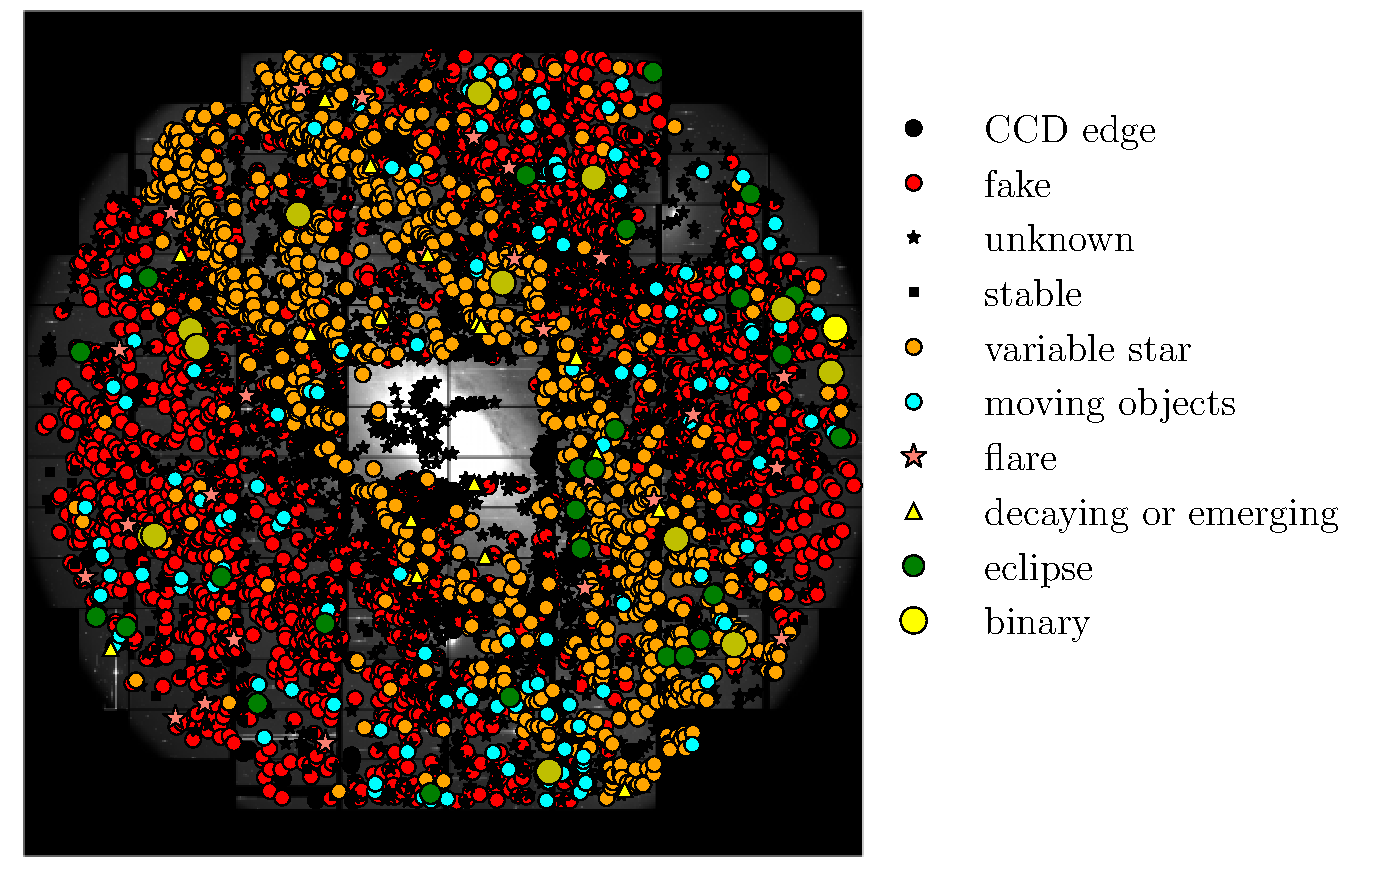
\includegraphics[width=8.55cm,clip]{pic/m31_fit6order.pdf}
%\includegraphics[width=8.55cm,clip]{pic/m31_fitspline.pdf}
%\caption{\small{Distribution of variable star candidates across the M31 region covered by 104 CCD chips. The right panel shows the distribution of variable candidates obtained when using the spline fitting method for background subtraction in each CCD chips (the default method of HSC pipeline). For this case we found about $1500$ candidates in total. The different color symbols are different types of variable candidates classified based on their light curves. Left panels displays the distribution of variable candidates obtained by using the 6 or 10-th order polynomial fitting method for each CCD chip (see text for details). For this case, we found about 11,000 candidates. For a particularly dense star region such as the bulge region or NGC205 region, our data processing method cannot properly work, and we cannot properly find candidates of variable stars in these regions. }}
%\label{fig:m31fit}
%\end{figure}
%
%
\item[(2)]{\it Star treatments on astrometry procedure}\\
%
One problem to note is that polynomial fitting often fails in mosaic procedure because 
only limited number of stars are used for the calculation. 
This problem is caused by the misdirection of cosmic rays as stars and the following misclassification of stars and galaxies due to the wrong measurement of PSF magnitudes. 
Therefore we applied object-size condition for PSF measurement, and abandon to use smaller candidates than default condition for images with seeing worse than $0.8''$ (default minimum size threshold is 0.9, and here changed to 1.3 for images with seeing $\sim1.2''$). 
At this moment we have succeeded to achieve a fairly accurate background subtraction using the polynomial fitting method. %, as shown in the left panel of Fig.~\ref{fig:inhomo}. 

\item[(3)]{\it Median background subtraction in the postage-stamp image around each candidate in the difference image}\\
As we described, we use the difference image to perform the PSF photometry of each time-variable candidate. However, the background subtraction is challenging and we often find a residual background mode around a candidate in the difference image. 
For example, if the difference image has a coherent negative counts around a candidate, the PSF photometry cannot work, because the PFS function is a decaying function with radius, asymptotically going to zero at large radii, and therefore a fitting of the PSF function to the difference image of the candidate with varying either positive or negative PFS flux parameter fails to reproduce the coherent background at large radii. 
To avoid a contamination of the residual background to the PSF photometry of a candidate, we measure the median background mode in $41 \times 41$ pixels around each candidate, subtract the median background from the postage-stamp image, and then perform the PSF photometry of the candidate in the difference image. 
%Fig.~\ref{fig:medisubpsf} shows the improvement in the PSF photometry due to the local background subtraction in the difference image. 
Based on the results, we used the median background subtraction around each candidate in the difference image as our default analysis. We succeed to discard more than $1000$ fake events from images with median subtraction. 
%
%\begin{figure}[t]
%\centering
%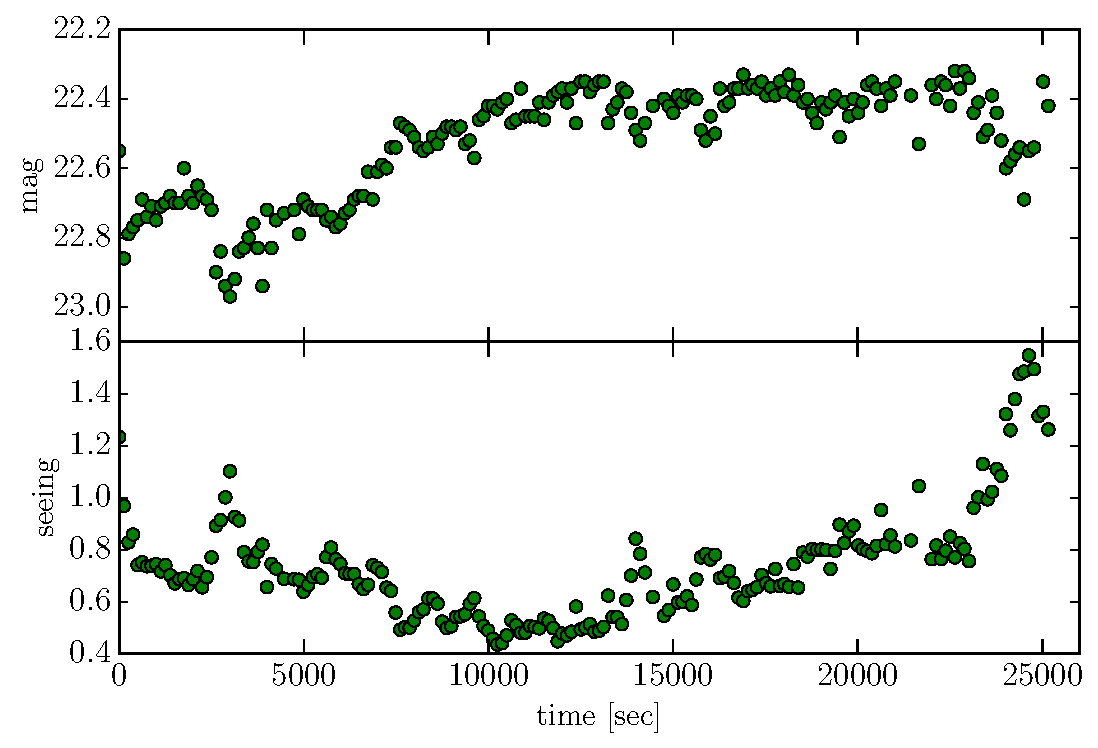
\includegraphics[width=10cm,clip]{pic/6,7_lightcurve_seeing.pdf}
%\caption{\small{A typical example of a fake candidate whose light curve (upper panel) has a clear correlation with the seeing variation (lower panel). The light curve has a sharp feature when the seeing size has a sudden change. }}
%\label{fig:corrcurve}
%\end{figure}
%
%
\item[(4)]{\it Fake candidates due to imperfect PSF matching in the image difference process}\\
\label{sec:unsolved}
Making the difference image or subtraction of the reference image from the target image requires a matching of different PSFs in the two images; more exactly, the HSC pipeline allows us to estimate the differential Kernel between the two PSFs so as to minimize residual images in the difference image. However, in reality, an imperfect PSF matching leaves residual fluxes of every object in the difference images. For some objects, the residual images might pass our detection threshold (S/N$>5$). Again, once a candidate passes the detection threshold in a single target image, we will study the light curve of the candidate over time. If this is the case, the light curve of such a fake object would correlate with the seeing size. In fact we are finding such fake candidates, as shown in Fig.~\ref{fig:corrcurve}. At the moment we think that such candidates are fake, if their light curve has a correlated shape with seeing variations in time. We have found about 1,000 such fake candidates, among 11,000 candidates. 
We simply made several ways tests in mosaic procedure by changing the group of image used to solve astrometry: $20$-frame grouping instead of $10$-frame (current analysis), or $1$-frame combined with one $30$ sec exposure image. 
The number of failure changed a bit but not drastically, because most candidates are detected in other time-frames. Therefore we skip this part to continue the analysis. 
%

\item[(5)]{\it Frequency of time variables for each type of variable stars}\\
\label{sec:sampling}
Our observation has unique property that many light curves has a peak $\sim11000$sec, around the best seeing period as displayed in Fig.~\ref{fig:corrcurve}. To see if these peaks are real, we imposed another detection conditions as following \S~\ref{sec:detecmethod}: first separate all images into even-odd groups using serial numbers. For each group we conducted the same detection tests as mentioned before; imposing selection conditions to the each stacked images that are composed of five time-sequential images. The final time-variable candidates are constructed from those which passed the conditions more than twice. Therefore we construct two sets of candidates which can imply for the variable stars with timescale longer than $20$ minutes. 

We compared the two results of even-odd tests with the candidates of $10$ minutes cadence, derived from \S~\ref{sec:detecmethod}. The candidates are be classified into three groups by the detection frequency and property: the first group including those detected in both even-odd cases, the second corresponding to those detected either in even-odd criteria, and the third constructed by those detected in only in previous analysis. The first group includes candidates that are feasible, most of which contain smooth curve or bumps; characteristics often seen in Cepheid stars or binary stars. 
Also the candidates categorized in the third group are likely to be fakes because many of them have noisy behavior or log-flux peaks. The unique event with peaks around the best seeing are contained in all three group sets, with almost the distribution for three cases. The same is true for events with sub-peaks correlated with the variation of seeing. Although we cannot get clear implications for the seeing-correlated events, this sampling rate test can work as a way to remove fake candidates. 
%
\end{itemize}



\section{Statistics and Selection Criteria-3}
\label{sec:res2}
%explain each selection criteria about shape characteristics of light curves (summary in table(s))
After an identification of secure time-variable stars and their light curve measurements, 
we search, from the host sample of candidates, for microlensing events due to primordial black holes that might exist in the halo regions of MW and M31. 


In this section, we describe our selection criterion for microlensing events with HSC-M31 data. 
Basically we applied the same selection criterion as we imposed in simulation: 
noise threshold and fitting condition. 


\subsection{Selection Criteria Statistics}
(naive explanation, how many events are rejected by each criteria)

We picked up significant points on the difference images, 
and choose 11,462 candidates by the number of detection. 
From these data we searched for microlensing candidates by imposing selection conditions in the following. 

The data we use consists of the reported time of each flux measurement (time), 
the photometric flux in the difference image, and the flux error. 

(In Kepler analysis they divide good fluxes by mean flux of the lightcurve 
which is calculated over 300 data points towards the center of the lightcurve, 
and subtract unity from this quantity to produce a fractional magnification lightcurve.)


The statistics and selection criteria are as follows:
%
\begin{itemize}
%
\item{fitting theoretical microlensing light curve}\\
Fitting theoretical microlensing light curve with counts in difference images, using errorbars from PSF photometry. 
Theoretical lightcurves in difference image can be described as:
%
\begin{equation}
\Delta F (t)= F_0 (A(t) - A(t_\mathrm{Ref}))
\label{eq:chi2dof}
\end{equation}
%
where $F_0$ is the constant parameter representing flux of the source star, 
$A(t)$ is the theoretical magnification, and  
$t_\mathrm{Ref}$ is the time around when 10 images for the reference image are taken. 
Theoretical microlensing light curve can be described %by Eq.~\ref{eq:diffmicro}, 
with three free parameters: $\beta$, $t_\mathrm{FWHM}$ (or $t_E$), and $F_0$,
and fixed parameter $t_\mathrm{max}$ from peak position. 
Free parameters can move in range $0<\beta<1$, $t_\mathrm{FWHM}<25000$sec, 
$0.5 \times (F_\mathrm{max}-F_\mathrm{base})/(A(u_\mathrm{min})-1)<1.5\times (F_\mathrm{max}-F_\mathrm{base})$ 
(the last parameter can be fixed), 
where we take $F_\mathrm{max}$ as $97.6\%$ percentile, and $F_\mathrm{base}$ as $15\%$ percentile of the time-variation flux. 

\item{fitting theoretical flare light curve}\\
In the same way as in microlensing lightcurves, magnification due to flare events can be described as
%
\begin{eqnarray}
A (t;B,C)=\left\{\begin{array}{ll}
 B \exp\left(-\frac{C (t-t_\mathrm{max})}{t_\mathrm{obsperiod}}\right) & (t>t_\mathrm{max})\\
 0  & (t<t_\mathrm{max})\\
\end{array}\right.
\label{eq:expflare}
\end{eqnarray}
%
Therefore free parameters are $B$ and $C$ so that $\Delta F (t)= A(t) - A(t_\mathrm{Ref})$, %(and baseline factor $BF$ so that $\Delta F (t)= A(t) - A(t_\mathrm{Ref})*BF$), 
and fixed parameter $t_\mathrm{max}$ from peak position. 
Free parameters can move in range $0.95<B<100$ and $C<1000$.  
%(and $0.5 <BF/(F_\mathrm{max}-F_\mathrm{base})<1.5$). 


\end{itemize}



%select those which have the best-fitting parameters by successful fitting. 

There exist some candidates which can pass the fitting conditions. 
As we have no criterion to clearly exclude such candidates, 
for now we just exclude them by comparing with image or eye-ball selections. 



\begin{table*}[t]%htbp[H]
\label{tab:selecond}
    \caption{Selection criteria}
    \begin{center}
   \begin{tabular}{ll}
      \hline %\hline
   \multicolumn{1}{l}{Statistic}&\multicolumn{1}{l}{Definition}\\
 \hline 
mlchi2dof & $\chi^2$ of fit to microlensing shape (divided by dof in Kepler's case)\\
fchi2dof & $\chi^2$ of fit to exponential flare shape (divided by dof in Kepler's case)\\ 
  \hline
  \hline
   \multicolumn{1}{l}{Selection Criterion}&\multicolumn{1}{l}{Purpose}\\
 \hline 
edgecriterion & remove bumps due to poor photometry\\
mlchi2dof$<0.75$ fchi2dof & microlensing fit better than flare fit\\
mlchi2dof$<$ ?? & microlensing fit is not too bad\\
asymmetry & remove short duration flare events\\
 \hline 
 \hline 
   \multicolumn{1}{l}{Statistic ($*$)}&\multicolumn{1}{l}{Definition}\\
 \hline 
$\langle f\rangle$ & average of $f_i$ over all good measurements in lightcurve\\
$A_i$ & flux$_i / \langle$flux$\rangle$\\
 \hline 
 \hline 
   \multicolumn{1}{l}{Selection Criterion ($*$)}&\multicolumn{1}{l}{Purpose}\\
 \hline 
edgecriterion & remove bumps due to poor photometry\\
 \hline 
   \label{table:counta}
  	\end{tabular}
	%\hspace{1 em}
	%\begin{tablenotes}
	%   \item {
         \tablecomments{\small ($*$) is only applied to Kepler's data }
	%\end{tablenotes}
	   \end{center}
   \end{table*}
%

\subsection{Background}
\subsubsection{Foreground Moving Objects in the M31 field-3}
events which passed selection criteria:comets

%\subsection{How many events?}summary


\section{Efficiency Calculation}
%After briefly reviewing basic properties of microlensing, 
We estimate an expected event rate of the microlensing for stars in M31 assuming that all the dark matter in halo regions of WM and M31 are PBHs of an assumed mass scale. 
We then use a simulation of the microlensing taking into account observational conditions and noise in order to estimate a detection efficiency of the microlensing events. 
Finally we estimate a number of source strs in M31 from the HSC data and then derive constraints on the abundance of PBHs from our search of the microlensing events. 
%primary shortcomings: lack of faint stars in the artificial star tests, which are used to add simulated events
%\begin{itemize}

\subsection{Milky Way and M31 halo models}
Next we model the mass distribution between M31 and us in the Milky Way Galaxy (MW). We assume that the dark matter distribution in each halo region of MW or M31 is given by an Navarro-Frenk-White (1997; hereafter NFW) model
%
\begin{equation}
\rho_\mathrm{NFW}(r)= \frac{\rho_{c}}{(r/r_{s})(1+r/r_{s})^2},
\label{eq:rho_nfwm}
\end{equation}
%
where $r_s$ is the scale radius and $\rho_c$ is the central density parameter. We adopt $\rho_{c}=1.40\times10^7$ $M_\odot$/kpc$^3$ and $r_s=16.1$ kpc for MW \citep{NestiSalucci:13}, and $\rho_{c}=4.05\times10^7$ $M_\odot$/kpc$^3$ and $r_s=8.18$ kpc for M31 \citep{Geehanetal:06}. These NFW profiles are shown to reproduce the observed rotation curves for MW and M31, respectively \citep{Klypinetal:02}. Taking into account the fact that the Earth (an observer) is placed at distance, $R_\oplus=8.5$kpc, from the MW center, the distance to a PBH at distance $D_L$ is given as 
%
\begin{equation}
r(D_\mathrm{L})=\sqrt{R_\oplus^2-2R_\oplus D_\mathrm{L}\cos(l)\cos(b)+D^2_\mathrm{L}}
\label{eq:dislens}
\end{equation}
%
where we assume the M31 position in Galactic coordinates as $l = 121.2^{\circ}$, $b = -21.6^{\circ}$ as mentioned in \S~\ref{sec:obsinfo}, the distance to M31 is $D_S=770$ kpc. 
%As for M31 halo profile we take into account the location of the targeting field (patch=2,6), which is $\sim6.7$ kpc away from the M31 center. The left panel of Fig.~\ref{fig:optdepth} shows the mass density profile as a function of distance from the Earth towards to M31, while the right panel shows the differential optical depth; integrating the curve up to a given distance, $xD_S$ (x axis) gives the optical depth. Thus optical depth for a star in M31 is $\tau\sim2\times10^{-6}$, that means that microlensing is very rare even for a single source star. However, we consider a millions of source stars in M31, we expect one event, if dark matter in halos of WM and M31 is made of PBHs. 

\subsection{microlensing rate}

In the following we calculate the expected number of microlensing events of PBHs per unit observation time -- i.e. expected even rate. 
If a source star moves across the Einstein radius, with a relative velocity on the sky, $v$, the time scale of microlensing is computed as
%
\begin{eqnarray}
T=\frac{2\sqrt{R^2_E-d^2}}{v} = \frac{2}{v} \sqrt{\frac{4GMD}{c^2}}\sqrt{1-\beta^2}=2t_0\sqrt{1-\beta^2}
\end{eqnarray}
%
where $R_E$ is the Einstein radius, $d$ is the shortest separation between star and PBH, and $\beta \equiv d/R_E$ is the impact parameter. 
To model the velocity component, we assume that each PBH in the halo region of MW or M31 moves according to the gravitational force of the interior mass at the PBH position: 
%
\begin{eqnarray}
V_\mathrm{halo}=\sqrt{\frac{GM_\mathrm{ran}(<r)}{r}}
\end{eqnarray}
%
where $M_\mathrm{ran}(<r)$ is the interior mass at radius r from the center, defined as
%
\begin{eqnarray}
M_\mathrm{ran}(<r)=4\pi\rho_sr^3_s\left[\ln(1+x)-\frac{x}{1+x}\right],\quad x=r/r_s
\end{eqnarray}
%
The typical time scale of microlensing can be estimated as
%
\begin{eqnarray}
\hat t =2t_0\simeq3.5{\rm hours} \left(\frac{M}{10^{-7}M_\odot}\right)^{\frac{1}{2}}\left(\frac{xDs}{100 \rm{kpc}}\right)^{\frac{1}{2}} \left(\frac{v}{200\rm{km/sec}}\right)^{-1}
\end{eqnarray}
%
Here we employed $V_\mathrm{halo}=200\rm{km/sec}$ for the typical velocity $v$, and considered PBHs with mass scale of $10^{-7}M_\odot$ and at distance 100kpc from us, as an example. 
Therefore the event rate of microlensing can be calculated as:
%
\begin{eqnarray}
\Gamma = \frac{4}{\pi}\frac{\tau}{\hat t}=0.91\left(\frac{M}{10^{-7}M_\odot}\right)^{-\frac{1}{2}}\left(\frac{xDs}{100 \rm{kpc}}\right)^{-\frac{1}{2}} \left(\frac{v}{200\rm{km/sec}}\right) [{\rm events/star/year}]
\end{eqnarray}
%
Next we take into account the velocity dispersion of PBH for precise modeling by assuming the Maxwell distribution: 
%
\begin{eqnarray}
f(v;r)=\frac{1}{\pi^{\frac{3}{2}}v^3_{c}}e^{-\frac{v^2}{V^2_{\rm halo}}}d^3 \vec{v}
\end{eqnarray}
%
Then the event rate can be expressed in the cylinder coordinate $d^3 v=v_r dv_x dv_r d\theta$ as: \citep{Griestetal:91}
%
\begin{eqnarray}
d\Gamma=\frac{\rho(r)}{M}f(v)v^2_r {\rm cos}\theta r_E dv_xdv_rd\theta d\alpha dx %\times u_T
\end{eqnarray}
%
where we assume that velocity direction of PBH is isotropic, and the mass density is consisted of 
NFW density profiles of MW and M31 halo. The integral can be calculated by substituting the variable as $\hat t=\frac{2R_E}{v_r}$. Therefore the event rate of microlensing is given by 
%
\begin{eqnarray}
\frac{d\Gamma}{d\hat t}=\frac{32D_S}{\hat t^4 Mv_c^2}\int^1_0 \rho(x) R^4_E e^{-\frac{4R^2_E}{\hat t^2 v^2_c}} dx \quad[\rm {events/star/year^2}],
\label{eq:evrate}
\end{eqnarray}
%
As for PBH in MW halo, we convert the lens distance $r$, originally expressed in the galactic coordinate ($l,b$) to the distance $x$ normalized by $D_S$ following the same way as in Eq.~\ref{eq:dislens}: $r^2=R^2_\oplus+(xD_S)^2-2R_\oplus xD_S{\cos}l{\cos}b$, where $R_\oplus$ is the distance from the solar system to the Galactic center. 
Fig.~\ref{fig:m31_eventrate} displays the event rate for lens PBH in either MW halo or M31 halo, and source stars in M31 ($D_S=770$ {kpc}). We calculated for cases with PBH mass of $M=10^{-7}$-$10^{-9}M_\odot$. The event rate for PBH mass $M$ can be calculated by scaling the $m=M_\odot$ case with $\sqrt{M}$ for horizontal axis and $M^{-1}$ for vertical axis. The left panel of Fig.~\ref{fig:m31_eventrate} shows the expected event rate from our data, showing that PBH in mass range $10^{-9}M_\odot$ - $10^{-7}M_\odot$ has maximum event rate in our sampling rate. Also one example of the contribution from PBHs in the two halos is given in the right panel. 
%
\begin{figure*}
\centering
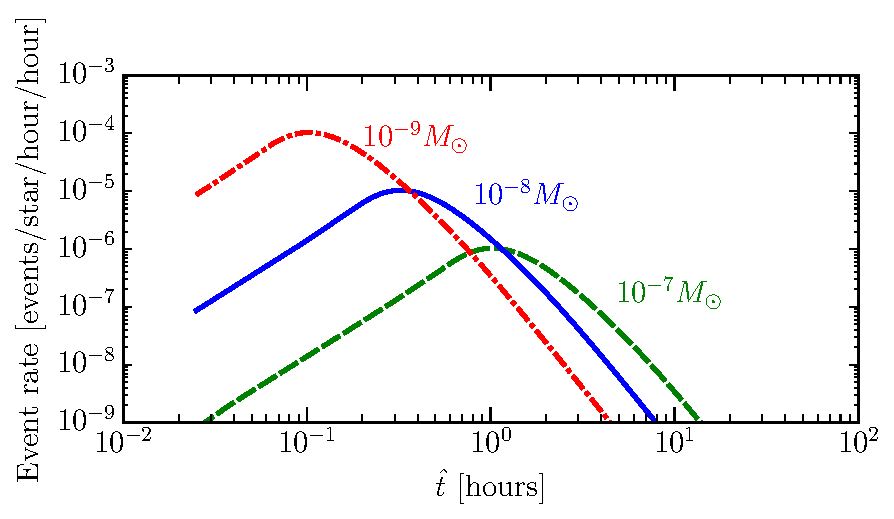
\includegraphics[width=0.45\textwidth]{pic/test_event_rate.pdf}
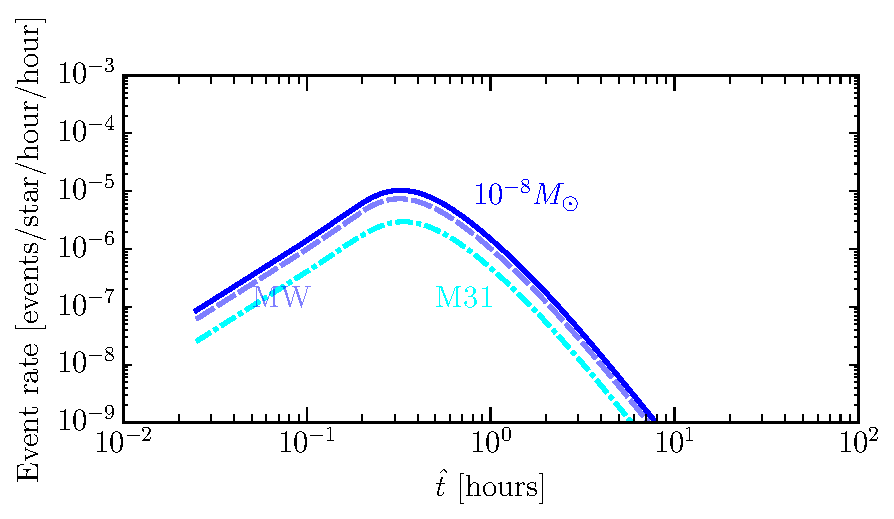
\includegraphics[width=0.45\textwidth]{pic/test_event_rate_8.pdf}
\caption{\small{
The differential event rate of microlensing due to PBHs, per unit observation time (hour), per a single star in M31, and per unit time scale of mirolensing (hour). The x-axis is the timescale of mcorlensing. Here the mass distribution of MW or M31 halo region is given by the NFW profile, all the dark matter is made of PBHs, and we considered PBHs with mass $10^{-9}, 10^{-8}$ or $10^{-7}M_\odot$, respectively. The lighter PBH has a shorter microlensing time scale. Right panel shows the relative contribution to the microlensing rate due to PBHs in either MW or M31 halo region. }}
\label{fig:m31_eventrate}
\end{figure*}
%
We can calculate the total event rate by integrating Eq.~\ref{eq:evrate} with $\hat t$:
%
\begin{eqnarray}
\Gamma=\int^\infty_0\frac{d\Gamma}{d\hat t}d\hat t=1.7\times10^{-6}\left(\frac{M}{10^{-7}M_\odot}\right)^{-\frac{1}{2}} \quad{\rm [events/star/hour]}%\times u_T 
\end{eqnarray}
%
The average timescale $\hat t$ is also given by 
%
\begin{eqnarray}
\langle \hat t \rangle=\frac{1}{\Gamma}\int^\infty_0\hat t\frac{d\Gamma}{d\hat t}d\hat t=1.8\left(\frac{M}{10^{-7}M_\odot}\right)^{\frac{1}{2}}\quad [{\rm hour}]
\end{eqnarray}



\subsection{Monte Carlo efficiency calculation}
%\item abundance limit
In this section we describe the current status of microlensing analysis. 
%Here we briefly summarize the results of our analysis using the data of one patch region alone, ``patch=2,6'', which is located between the halo and disk regions of M31.

\begin{itemize}
\item[(1)]{\it Null test}\\
%\subsection{Null test}
\label{sec:nullt}
A detection efficiency of microlensing event is sensitive to the noise properties in the difference image. To estimate the noise field in the difference image difference, we use the following method. We first randomly select 1000 points in a bank region of the difference image (excluding the region of a candidate). Second we make the PSF photometry of the random points. Then we compute the variance of the PSF magnitude, which gives us an estimate of the noise field in the patch. Note that, in estimating the noise variance, we performed the median background subtraction in the difference image of the patch as we described above. 

Fig.~\ref{fig:nulltest} shows the case with noise threshold $1\sigma$, $3\sigma$ and $5\sigma$ flux converted to magnitude unit. On each panel, square symbols are tests with difference images constructed from time-sequentially five-stacked images, and circle marks are tests with difference images of each visit. We used the former images for detection and the latter images for photometry. As expected, the noise gets smaller when we stacked five images than cases with each image. Also it is proved by comparing the upper and lower panels that the threshold gets smaller for the measurement with local median subtraction. 
The results imply that stars with base magnitude $25$ or $26$ magnitude are around the borderline for $5$ or $3$ sigma noise thresholds respectively. 
%
\begin{figure*}
\centering
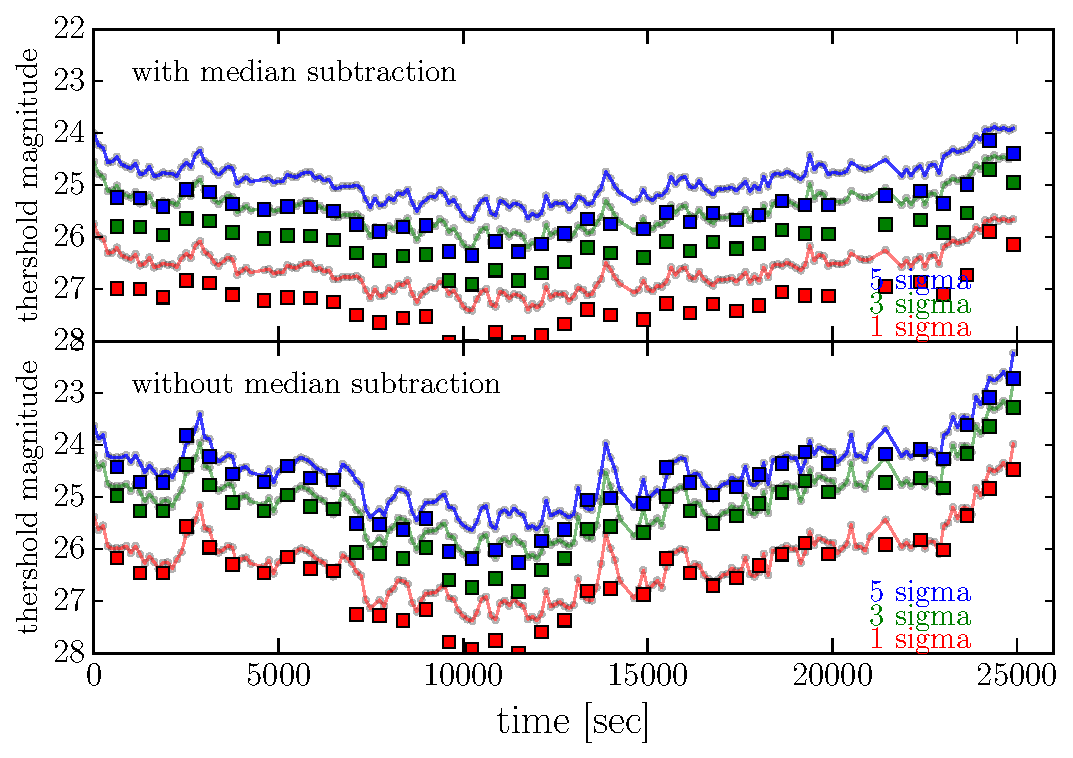
\includegraphics[width=0.6\textwidth]{pic/threshold_seeing_coadd_both.pdf}
%\includegraphics[width=7.cm,clip]{pic/randd.pdf}
\caption{\small{An estimation of noise variance in the difference image. Here we show the results for the difference image of patch=2,6 as an example. We randomly select 1000 points in a blank region of the difference image (as shown in the right panel), measure the PSF magnitude of each point and then estimate the variance of PSF magnitude. The left panels shows the noise variance, 1, 3 or 5sigma,  as a function of observation time.  The square symbols show the results when using the coadd images of 5 time-sequential exposures for the difference image. The circle symbols, connected by the line, are the results for each exposure. The difference in the upper and lower plots is with or without the median background subtraction of the difference image. }}
\label{fig:nulltest}
\end{figure*}
%

\item[(2)]{\it Magnification threshold from photometry error}\\ 
Until now, we define magnification threshold of microlensing event as $A>1.34$ in this experiment. 
To see if the threshold is proper, we looked into the uncertainty of PSF photometry. 
Fig.~\ref{fig:rsm} shows the magnitude or PSF flux error distribution of field stars on the reference image. The error distribution indicates that stars with PSF flux $\sim0.6$[ADU] at 90 sec exposure, corresponding to stars brighter than $25.8$ mag can barely probe $A>1.34$ magnification. Although this flux error comes from reference image and the measurements on difference images might have different effect, we conclude that $3\sigma$ threshold Fig.~\ref{fig:nulltest} can work as noise threshold by comparing the result in the upper panel. 
%
\begin{figure*}
\centering
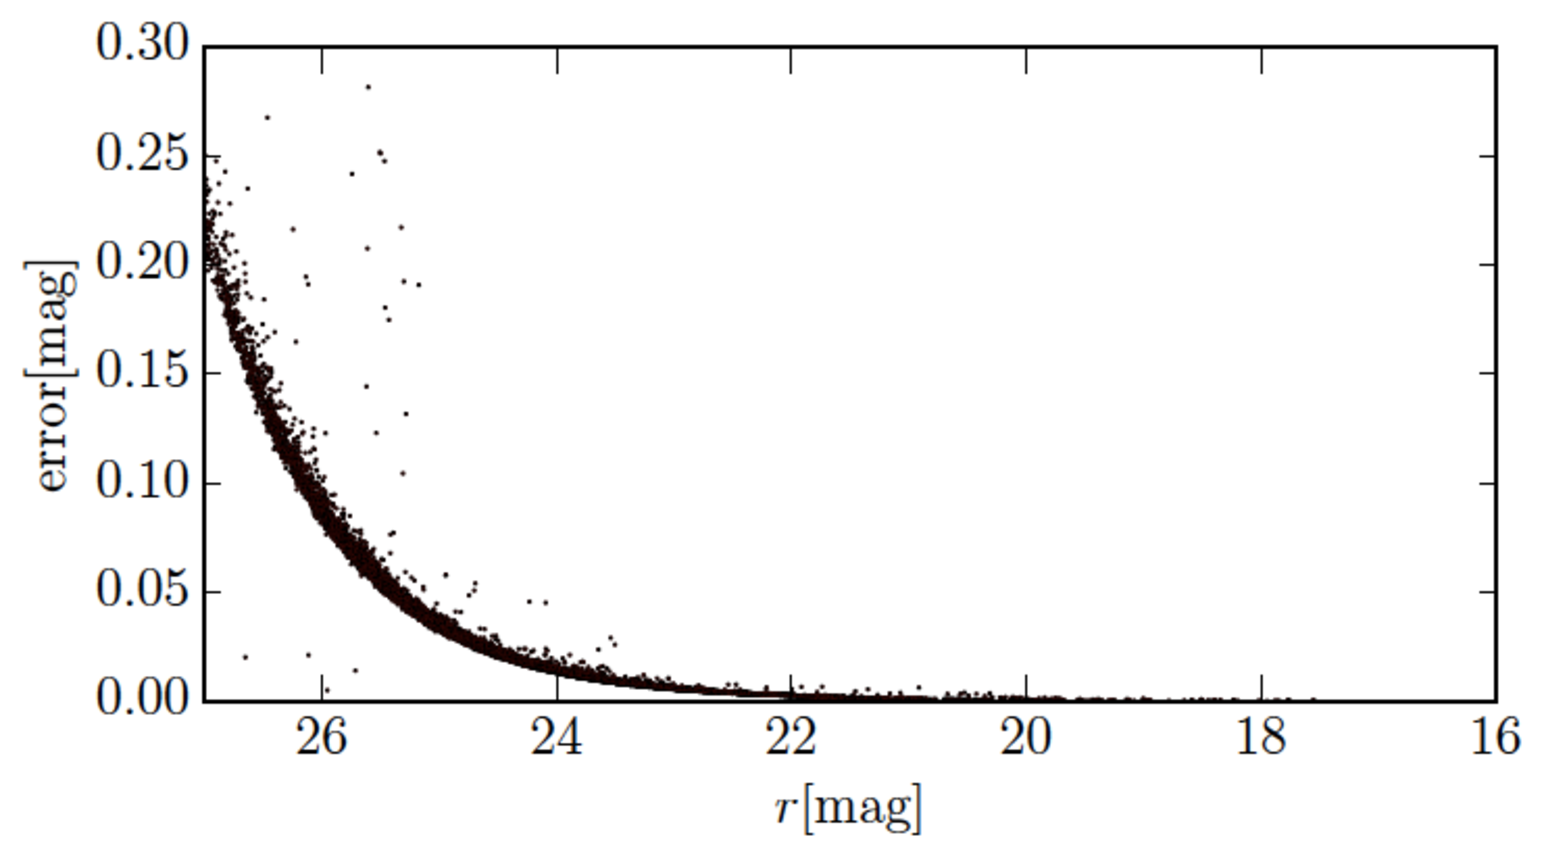
\includegraphics[width=0.45\textwidth]{pic/2,6_err_r.pdf}
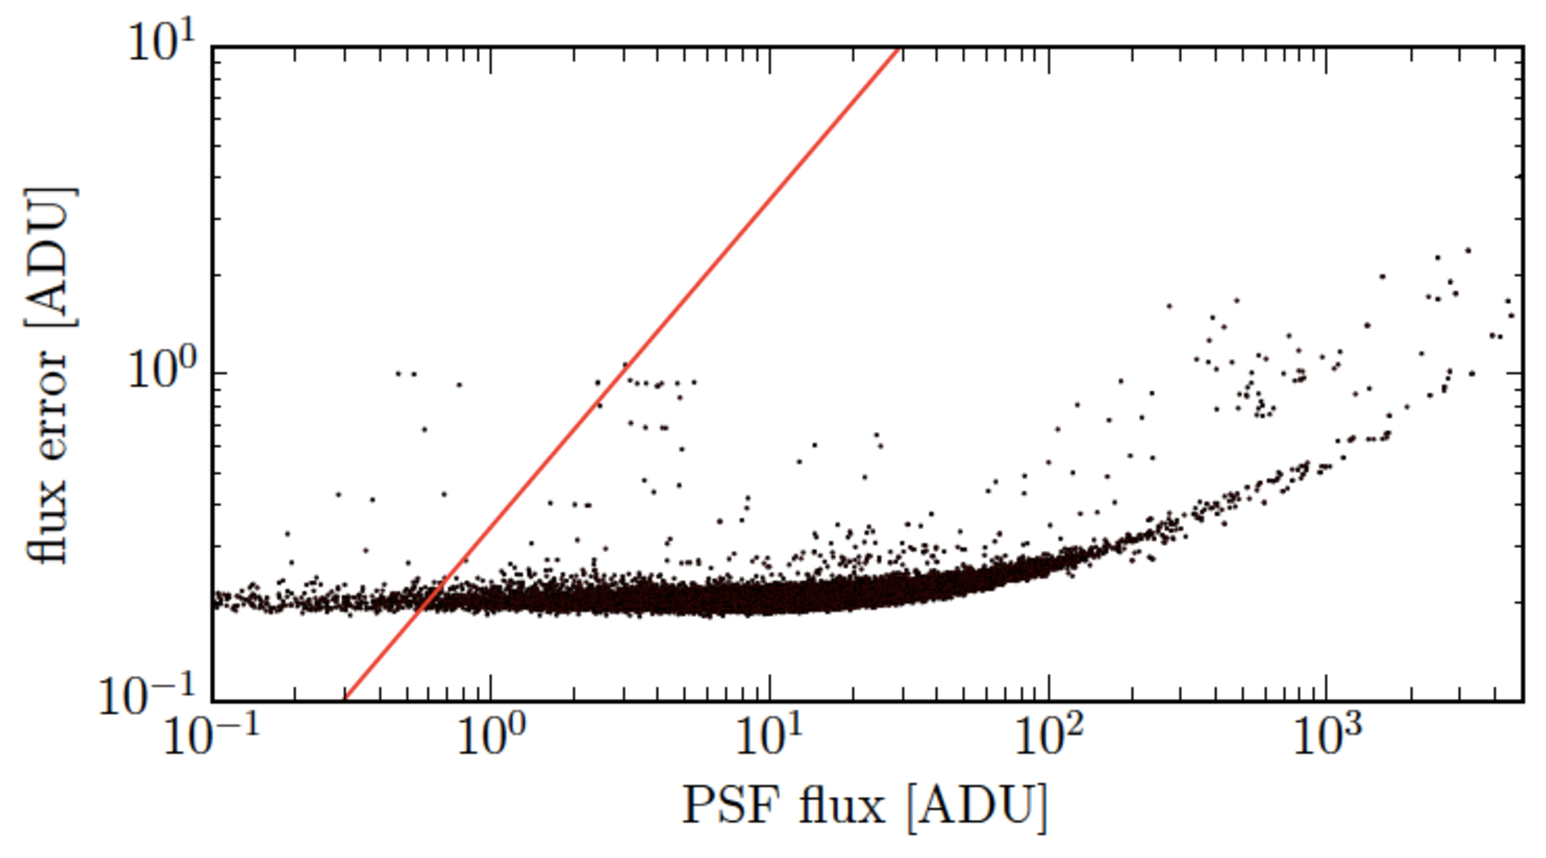
\includegraphics[width=0.45\textwidth]{pic/2,6_err_r_flux.pdf}
\caption{\small{Uncertainty of star flux in our data. {Left panel} shows PSF magnitude errors of each star. The star samples are constructed from the star catalog of the targeting field (the detail of catalog property is described in \S~\ref{sec:snumber}). {Right panel} displays the PSF flux error in the unit of ADU for the same star samples of 90 sec exposure. The red line corresponds to the border line that flux error is above or under 0.34 times of PSF flux, which indicates that stars with PSF flux larger than the line can overcome the magnification condition: $A>1.34$. The error distribution indicates that stars with PSF flux $\sim0.6$[ADU] at 90 sec exposure, corresponding to stars brighter than $25.8$ mag can barely probe $A>1.34$ magnification.  }}
\label{fig:rsm}
\end{figure*}
%

\item[(3)]{\it Detection efficiency}\\
We have so far employed the formal definition of microlensing that a source star should be within the Einstein radius of a foreground PBH, corresponding to the magnification $A>1.34$. However, it is unclear whether the lensed source can be detected by our observation. The detection threshold should depends on the intrinsic brightness of a source star, the noise field in the difference image, the amount of lensing magnification, and the time-scale of light curve in order for us to capture the light curve within our observation time duration (7 hours).  
Thus we need to properly estimate the detection efficiency. 
Detection efficiency is simply given by $\epsilon(\hat t_i)\equiv$(The number of detected events)/(Total number of events occurred). 
In the following we discuss the two kinds of tests performed for efficient estimation; 
one with simulated light curves, and the other with embedded candidates in the image. 
\begin{itemize}
	\item[a)]{\it efficiency test with light curve simulations}\\
	First we studied the event property with simulation of microlensing light curves. 
	The theoretical light curves are constructed by mimicking our detection method as in \S~\ref{sec:obstrans}; 
	we simulated the time-variated flux of each event in the difference images. 
	For each event we change the conditions using three parameters; 
	Einstein time scale $t_{E}$, impact parameter $\beta$, and 
	the time when maximum amplification occurs $t_{\rm max}$. 
	Note that impact parameter is decided to meet the condition $0<\beta<1$, and 
	typical time scale $t_\mathrm{FWHM}$ and maximum flux parameter $\Delta F_\mathrm{max}$ are  
	calculated from the above parameters. 
	Also for excess noise parameter, we correct for the base flux 
	in the same way as derived from image difference technique; 
	the reference magnitude is constructed from the average of 10 best-seeing frames.
	
	By assuming cases with the PBH mass $10^{-7}M_\odot$, 
	we created every $1000$ events for different $t_\mathrm{FWHM}$, and counted the number of events 
	when more than three data points continuously passed the $3\sigma$ noise threshold as in the upper panel of Fig.~\ref{fig:nulltest}. 
	For the event time scale we take $5$ minutes for the minimum so as to have more than three data points 
	above the noise threshold.  
	We also take $11$ hours as the maximum timescale because events longer than this timescale have 
	longer half-width-half-maximum than the total observational time, which makes it difficult to discriminate the 
	microlensing event with other variable star such as Cepheid variable stars. 
	On each light curve we add the flux noise to the simulated microlensing flux 
	measured at the random point in the difference image. 
	%One example of simulated light curve is given in Fig.~\ref{fig:fakecurve}. 
	Note that $1000$ points are selected by avoiding the CCD edge region, 
        because we cannot measure the flux property at that point. 

	Fig.~\ref{fig:efficiencyeach} describes the detection efficiency for events with different 
	timescale and source magnitudes. 
	There exist drastic drops of detection efficiencies for events longer than the observational period, longer than 7 hours. 
	One reason for this effect is that fitting by theoretical microlensing light curve does not work for these events because of unstable baseline. 
	For events with time scale shorter than observational period, 
	the detection efficiencies are almost constant for stars brighter than $23$ magnitude. 
	On the other hand, when the source stars fainter than $24$ magnitude have lower detection efficiency, which indicates that 
	faint stars need some specification to pass the threshold. 
	Another characteristics of detection efficiency is that it takes lower value for events with shorter time scale. 
	This is reasonable for shorter events because 
	it is hard for them to pass the threshold when magnification peak falls in high noise period.  
%
\begin{figure*}
\centering
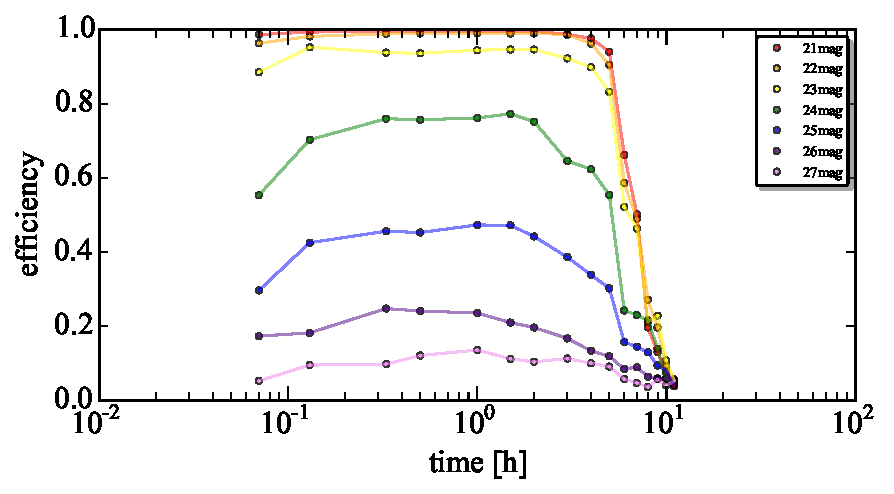
\includegraphics[width=0.6\textwidth]{pic/efficiency_eachmag.pdf}
\caption{\small{ The detection efficiency estimated from light curve simulations taking into account the noise field in each difference image of 194 target images we used for the analysis (see text for details). Here we generated Monte Carlo simulations of microlensing events randomly varying the two parameters: the impact parameter (or maximum lensing magnification) and the FWHM time scale parameter, for source stars of a fixed magnitude as indicated by legend. The x-axis is the microlensing time scale. The detection efficiency for each source magnitude is estimated from 1,000 realizations.}}
\label{fig:efficiencyeach}
\end{figure*}
%
	We also looked into parameter properties that meet the selection conditions, just by fitting the simulated light curves with theoretical microlensing prediction. To simplify the case, we fit the light curves with $t_{\rm FWHM}$ and $\beta$ parameters, and fix $t_{\rm max}$ as the time of maximum peak during observation.   
	Fig.~\ref{fig:efficiencypara} shows the best-fit parameter distribution derived from simulated events of $24$ magnitude. This figure indicates that $\beta$ has some threshold for all the time scale, suggesting that events are detected only when source stars come close enough to the center of PBH lens in the line of sight.  
%
\begin{figure*}
\centering
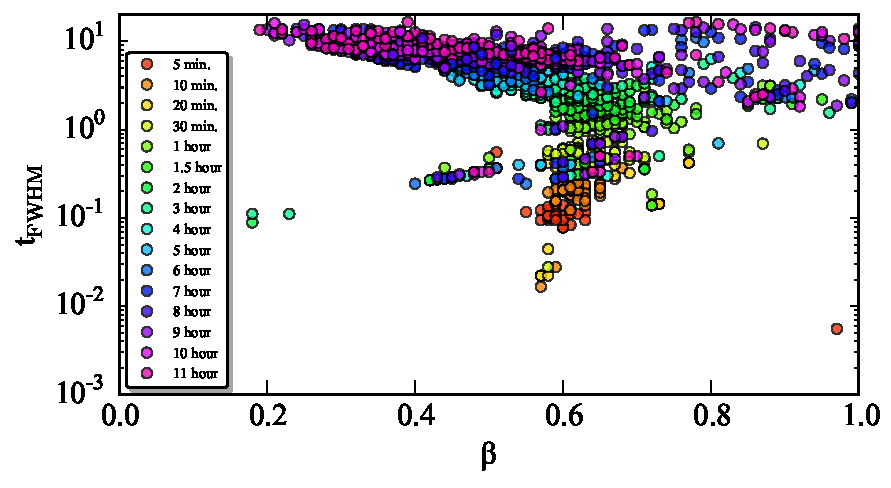
\includegraphics[width=0.6\textwidth]{pic/efficiency_parameter.pdf}
\caption{\small{ The distribution of microlensing parameters for source stars with $24$ magnitude.  Each point is derived by the fitting of a simulated light curve. We tested 400 events for every event with different time scale. Here we perform the fitting with two parameters; impact parameter $\beta$ and timescale parameter $t_\mathrm{FWHM}$, and the maximum time of the event $t_\mathrm{max}$ is fixed at the time of maximum flux. }}
\label{fig:efficiencypara}
\end{figure*}
%
        \item[b)]{\it efficiency test with fake object simulations}\\
	We performed another test to estimate the detection efficiency in more concrete way; 
	burying fake microlensing stars in the observational CCD imaging data and proceed the same 
	analysis as mentioned in \S~\ref{sec:obstrans}. 
	Thus we can include the PSF smoothing effect 
	followed by the stacking or subtracting procedures, which might 
	affect the flux count in the output images. 
	Also we can take advantage of the same detection condition, including shape conditions or 
	the residual condition, which are all neglected in the light curve simulations. 
	
	Fake stars simulations are all performed by $fake$-$pipe$ module installed in HSC-pipe, which 
	enables one to bury fake stars in CCD reduced image by means of PSF information in that field.  
	In order to study the detection efficiency we buried $1000$ stars at random position, 
	avoiding the CCD edge regions. 
	The flux variation due to microlensing effect are calculated 
	in the same way as we performed in the light curve simulation; 
	taking $t_{E}$, $\beta$, and $t_{\rm max}$ as free parameters. 
	
	Fig.~\ref{fig:ebury} shows the comparison of detection efficiency derived from the different tests: 
	light curve simulation, light curve simulation with successful fitting, and burying tests. 
	Among the results from source stars of $24$ magnitude, 
	burying test implies slightly smaller efficiency compared to tests with simulated light curve. 
	This might come from the additional performance of HSC-pipe for the subtraction and detection  
	in the difference images. 
	In the following we adopt the implications from simulated light curves %burying tests, 
	although the estimation is very optimistic. 
	%	 	
\begin{figure*}
\centering
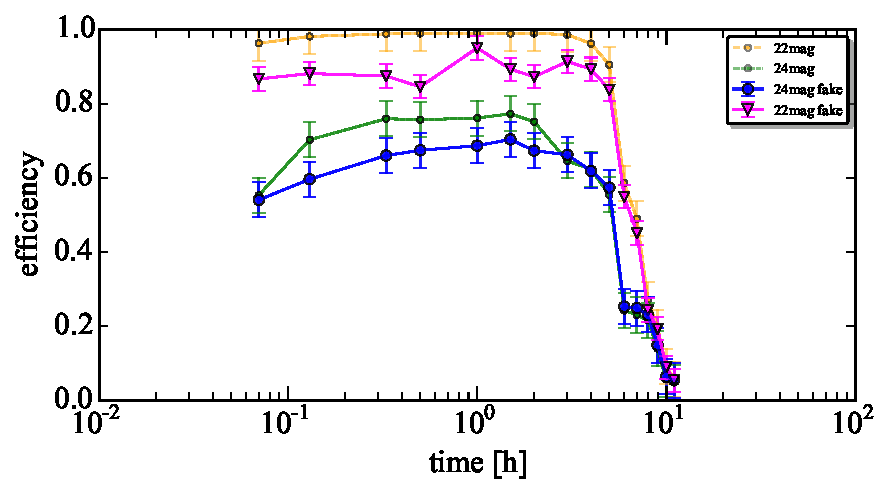
\includegraphics[width=0.6\textwidth]{pic/efficiency_fitting.pdf}
\caption{\small{ Comparison of detection efficiency from different tests, focusing on  the results from stars with $22$ and $24$ magnitude (All the error-bars come from Poisson noise).  Small circles show the results from light curve simulations (the same as shown in Fig.~\ref{fig:efficiencyeach}), and large marks represent the results from fake image simulations, where we inject fake point source in the real image and performed the same analysis of microlensing search. }}
\label{fig:ebury}
\end{figure*}
%
\end{itemize}


\end{itemize}


\subsection{Star number counts in HSC M31 data}
%mention about our weakness ..
\label{sec:snumber}
The expected number of microlensing events in a field greatly depends on the number of source stars in that field (see the detail in \S~\ref{sec:constraint}). However in M31 field, it is hard to estimate the star number counts because multiple stars are expected to exist in one pixel and cannot be resolved;  
the situation so-called pixel lensing regime. In the following we describe our test in the targeting field to seek for better estimation way of the star number counts . 



In the first step we take a look at the star property in the targeting field 
by taking advantage of the reference image with seeings $\sim 0.45$. 
Even in the pixel lensing regime, stars in M31 halo region are almost resolved 
with the help of high resolution.  


We conclude that the peak catalog can basically work as star catalog of the targeting field. We also consider that the number counts can be more safely estimated by extending the threshold magnitude up to around $26$ [mag] with monotonically increased counts following empirical luminosity function and the halo region case. 
As for distribution of number counts, star catalogs tend to have log-declined slope in the fainter end while peak catalogs have magnitude threshold, both of which is inconsistent with the monotonic increase tendency suggested by empirical star luminosity function \citep[ex.][]{MamonSoneira:82}. 
We also calculate the sum of pixel count with PSF count from catalog, with the sum of the whole pixel counts in the image. The result indicates that the total PSF count calculated with peak positions is in the same order of total pixel count. 

Note that there exists a conventional way to correct the field magnitude 
by combining extinction map and empirical luminosity function. 
Magnitude property differs due to the dust distribution in the field, 
which redden the magnitude in homogeneously even within the same galaxy, 
and might cause a systematic bias and large uncertainty. 
Extinction map can be constructed by studying the sub-field properties;  
taking advantage of the color-magnitude distribution 
of Red Clump Giants in that field (Paczy${\rm \acute{n}}$ski et al. 1999). 
We draw color-magnitude diagram by $g$-band and $r$-band star catalog. %as in Fig.~\ref{fig:cdm}, 
and searched for  red giants such as Asymptotic Giant Branch (AGB) stars 
by \citet{Kurucz:93} air model. 
However, due to the magnitude cut in the star catalog 
we could not estimate the property of Red-Clump stars from the diagram. 

As for magnitude bias, we take into account extinction effect 
when modeling the M31 halo density profile, because 
inhomogeneity can largely bias the microlensing result especially for M31 halo-lensing case. 
Currently for the self-lensing case we do not allow for the extinction effect 
because Andromeda Galaxy is 20 degree away from the galactic plane, 
which makes the inhomogenity small enough compared to M31's contribution.  



%start comments
\begin{comment}
In the first step we take a look at the star property in the targeting field 
by taking advantage of the reference image with seeings $\sim 0.45$. 
Even in the pixel lensing regime, stars in M31 halo region are almost resolved 
with the help of high resolution.  
Therefore we constructed two kinds of star catalogs by HSC-pipe,   
and look into the properties. 
The properties of two catalog are summarized as follows: 
%
\begin{itemize}
\item[(1)]{{\it Star catalog constructed by HSC-pipe} --- containing stars detected by $multiband.py$ programs, which performs auto-debrending procedures. Photometry was performed on fixed point with PSF magnitude. Due to the failure of the program, stars are selected only from partial regions. }
\item[(2)]{{\it Peak catalog} --- including the positions of auto-detected peaks by HSC-pipe. For each peak we perform PSF photometry. The distribution of peaks is spread all over the image, but some magnitude threshold might prevent the detection of dark candidates. }
\end{itemize}
%
\begin{figure*}
\centering
\includegraphics[width=0.3\textwidth]{pic/1,5_hist_r_psf_peak_try2.pdf}
\includegraphics[width=0.3\textwidth]{pic/2,6_hist_r_psf_peak_try2.pdf}
\includegraphics[width=0.3\textwidth]{pic/4,4_hist_r_psf_peak_try2.pdf}
\caption{\small{
The number counts of stars in some patch regions of M31. Here we employ 0.1 mag for the magnitude binning, and considered two different catalogs of stars. The blue histogram shows the number counts for stars that are identified by the HSC pipeline based on the imposed conditions. The green histogram shows the number counts for "peaks" that are identified from local peaks in the flux field in each image. {Left panel} is from M31-halo region (patch=1,5), {middle panel} is from halo-disk region corresponding to the targeting field in this section (patch=2,6), and {right panel} is from bulge region (patch=4,4). }} 
\label{fig:histmag}
\end{figure*}
%
Fig.~\ref{fig:histmag} shows the magnitude distribution of stars for three regions: halo region, targeting region in-between halo and disk, and bulge region. Basically two catalogs have similar distribution, but the number counts from star catalog tends to be lower than that of peak catalog due to the lack of analyzed region in star catalog. Also for distribution of number counts, star catalogs tend to have log-declined slope in the fainter end while peak catalogs have magnitude threshold, both of which is inconsistent with the monotonic increase tendency suggested by empirical star luminosity function \citep[ex.][]{MamonSoneira:82}. 
We also calculate the sum of pixel count with PSF count from catalog, with the sum of the whole pixel counts in the image. The result is summarized in the following table, which indicates that the total PSF count calculated with peak positions is in the same order of total pixel count. 

From the above pixel count result, we conclude that the peak catalog can basically work as star catalog of the targeting field. We also consider that the number counts can be more safely estimated by extending the threshold magnitude up to around $26$ [mag] with monotonically increased counts following empirical luminosity function and the halo region case (in the left panel of Fig.~\ref{fig:histmag}). 
%
\begin{figure*}
\centering
\includegraphics[width=0.45\textwidth]{pic/location_number_lin_ave.pdf}
\includegraphics[width=0.45\textwidth]{pic/location_number_lin_peak.pdf}
\caption{\small{Flux and peak number counts distributions of HSC-M31 region. 
The rectangles in each map show analyzed regions: 
blue rectangle is M31-halo region (patch=1,5), cyan one is halo-disk region corresponding 
to the targeting field in this section (patch=2,6), 
green one is disk region (patch=3,8), and red one is from bulge region (patch=4,4). 
Both panels are plotted with linear color scales; white side of the bottom color bars means larger and black means smaller. 
{Left panel} shows the distribution of the average flux counts in the unit of patch, 
suggesting the existence of very bright patches around M31 bulge and NGC205. 
{Right panel} shows the distribution of the number density of peaks. The number counts of peaks is 
smaller for disk and bulge regions, which is inconsistent with higher pixel counts 
compared to halo region. 
}} \label{fig:dist}
\end{figure*}
%


\begin{table*}[t]%htbp[H]
    \caption{Properties of flux count and star number counts for sub-regions of HSC-M31\label{tab:m31-table}}
    \begin{center}
   \begin{tabular}{lcccccc}
      \hline %\hline
   \multicolumn{1}{l}{Region}&\multicolumn{1}{l}{$\#$patch} & \multicolumn{1}{l}{Total pixel count} & \multicolumn{1}{l}{Total peak count}  &
    \multicolumn{1}{c}{Total Star count} &\multicolumn{1}{l}{$\#$peaks}&\multicolumn{1}{l}{$\#$stars}\\
 \hline 
%Halo &0,4 &$97626.3$ & $81684.8$	&$10839.4$ & 5365 & 2099 \\
Halo &1,5 &$3.11\times10^6$ & $2.34\times10^6$	&$1.52\times10^5$ & 147387 & 14807 \\
Halo-disk &2,6  &$4.71\times10^6$ &$5.70\times10^6$ &$9.66\times10^5$& 136933 & 40976  \\
Disk &3,8  &$4.87\times10^6$ &$6.12\times10^6$ &$8.86\times10^5$& 119188 & 32694  \\
Bulge &4,4  &$5.91\times10^6$ &$1.24\times10^6$ &$2.32\times10^6$& 124096 & 46904  \\
  \hline
   \label{table:counta}
  	\end{tabular}
	%\hspace{1 em}
	%\begin{tablenotes}
	%   \item {
         \tablecomments{\small {\it Note:} Total pixel count property in different regions; M31-halo region (patch=1,5), 
halo-disk region corresponding to the targeting field in this section (patch=2,6), 
disk region (patch=3,8),  
and bulge region (patch=4,4). 	   
The total PSF count of the targeting region (patch=2,6) derived from peaks 
	   is in the same order as total pixel count of that image. }
	%\end{tablenotes}
	   \end{center}
   \end{table*}
%
Note that there exists a conventional way to correct the field magnitude 
by combining extinction map and empirical luminosity function. 
Magnitude property differs due to the dust distribution in the field, 
which redden the magnitude in homogeneously even within the same galaxy, 
and might cause a systematic bias and large uncertainty. 
Extinction map can be constructed by studying the sub-field properties;  
taking advantage of the color-magnitude distribution 
of Red Clump Giants in that field (Paczy${\rm \acute{n}}$ski et al. 1999). 
We draw color-magnitude diagram by $g$-band and $r$-band star catalog as in Fig.~\ref{fig:cdm}, 
and searched for  red giants such as Asymptotic Giant Branch (AGB) stars 
by \citet{Kurucz:93} air model. 
However, due to the magnitude cut in the star catalog 
we could not estimate the property of Red-Clump stars from the diagram. 

As for magnitude bias, we take into account extinction effect 
when modeling the M31 halo density profile, because 
inhomogeneity can largely bias the microlensing result especially for M31 halo-lensing case. 
Currently for the self-lensing case we do not allow for the extinction effect 
because Andromeda Galaxy is 20 degree away from the galactic plane, 
which makes the inhomogenity small enough compared to M31's contribution.  
%
\begin{figure}
\centering
\includegraphics[width=0.3\textwidth]{pic/cmd2.pdf}
\includegraphics[width=0.3\textwidth]{pic/cmd.pdf}
\includegraphics[width=0.3\textwidth]{pic/cmd3.pdf}
\caption{\small{Color-magnitude diagram for three regions constructed from star catalog: halo region (patch=1,5), targeting region in-between halo and disk (patch=2,6), and bulge region (patch=4,4) from left to right. Red giants in M31 are expected to show up around $g_0\sim25$mag and $(g-r)\sim1.0$ region 
(corresponding to yellow box; red giants in MW is expected in blue-box region). However, we cannot study the expected clumpy property due to the failure in the debrending process of $multiband.py$ program, 
which prevent the statistical study of the stars. }} 
\label{fig:cdm}
\end{figure}

\end{comment}
%comments end


\subsection{equations of expected number of event detection} %(this sectioncan be moved to front)
%\end{itemize}
%\section{Detectable parameters-2}
%Also of interest..
\label{sec:constraint}
From the all the results above, 
we can derive the mass fraction of PBHs occupying the entire halo. 
In the following we estimate the fraction by null detection of microlensing event at the targeting field (patch=2,6). 
First we consider the expected number of microlensing events, taking into 
the account of the detection efficiency we estimated above.
Here we assume the halo model of Milky Way galaxy as the standard exponential model. %, ...???
Then the event rate can be estimated as:
%
\begin{eqnarray}
\frac{d\Gamma}{d\hat t}=\frac{32D_S}{\hat t^4 Mv_c^2}\int^1_0 \rho(x) R^4_E e^{-\frac{4R^2_E}{\hat t^2 v^2_c}} dx \quad[\rm {events/star/yr^2}]\nonumber
\end{eqnarray}
%
where $M$ is the mass of PBHs, and $\hat t$ is the duration time of the microlensing event. 
%
%\begin{figure}[t]
%\centering
%\includegraphics[width=8.cm,clip]{pic/test_number_of_expected_event_m31.pdf}
%\includegraphics[width=8.cm,clip]{pic/test_number_of_expected_event_m31_2.pdf}
%\caption{\small{Expected number of microlensing events for source stars in the patch=2,6 region, as a function of PBH mass in the horizontal axis. The right panel shows an upper limit on the abundance of PBHs assuming we don't have any secure candidate of PBH microlensing (no detection). To convert no detection to the upper limit, we assumed that some portion of dark matter in the halos regions of MW and M31 is made of PBHs, parameterized by $\Omega_\mathrm{PBH}/\Omega_\mathrm{DM}$ in the vertical axis. }}
%\label{fig:m31_number_exp}
%\end{figure}
%
In the case where MACHO has flat mass distribution like delta function, 
the expected number of events $N_{\rm exp}$ with MACHOs of mass $M$ is estimated as
the integral of the event rate via $\hat t$, 
multiplied by duration time and the total exposure:
%
\begin{eqnarray}
N_{\rm exp}(M)=E\int^{\infty}_0 \frac{d\Gamma}{d\hat t}(\hat t,M)\epsilon(\hat t)d\hat t
\end{eqnarray}
%
where $E$ is the multiplication of the number of stars and the total observational period in the unit [star$\times$years]. 
By assuming that the length of our observation is $7$ hours and the targeting field (patch=2,6) contains $1.4\times10^5$ stars, 
We can calculate the expected number of events as in the Table (TBD). %left panel of Fig.~\ref{fig:m31_number_exp}. 




\section{Limits on PBH Dark Matter and Discussion-3}
%\section{Implications}
%comparison with other data?
\subsection{Errors in Present Analysis}
The number of stars in the field..?
%\subsection{Likelihood Analysis and Dark Matter}
%\subsubsection{Microlensing Rate}
%\subsubsection{Milky Way and M31 Models}
\subsubsection{PBH Halo Fraction and Mass}
From this result we estimate the mass fraction of PBH to dark matter. 
Assuming that the event has Poisson distribution, 
the upper limit where less than one event happens in 95\% confidential level is $N_{\rm exp}<3.7$. 
Then we can put upper limit on the dark matter fraction of PBHs in the total dark matter halo as:
%
\begin{eqnarray}
f_{\rm lim}(M)=\frac{3.7}{N_{\rm exp}(M)}
\end{eqnarray}
%
Note that this upper limit holds whichever the lens body resides in the Milky Way halo or not. 
The current limit from four-patch fields 
from our analysis is presented in the right panel of Fig.~\ref{fig:m31_number_exp}.  
We also display the constraint expected from the whole field of view by the fact that 
total star counts from peak statics are $6,843,112$. 
%
\begin{figure*}
\centering
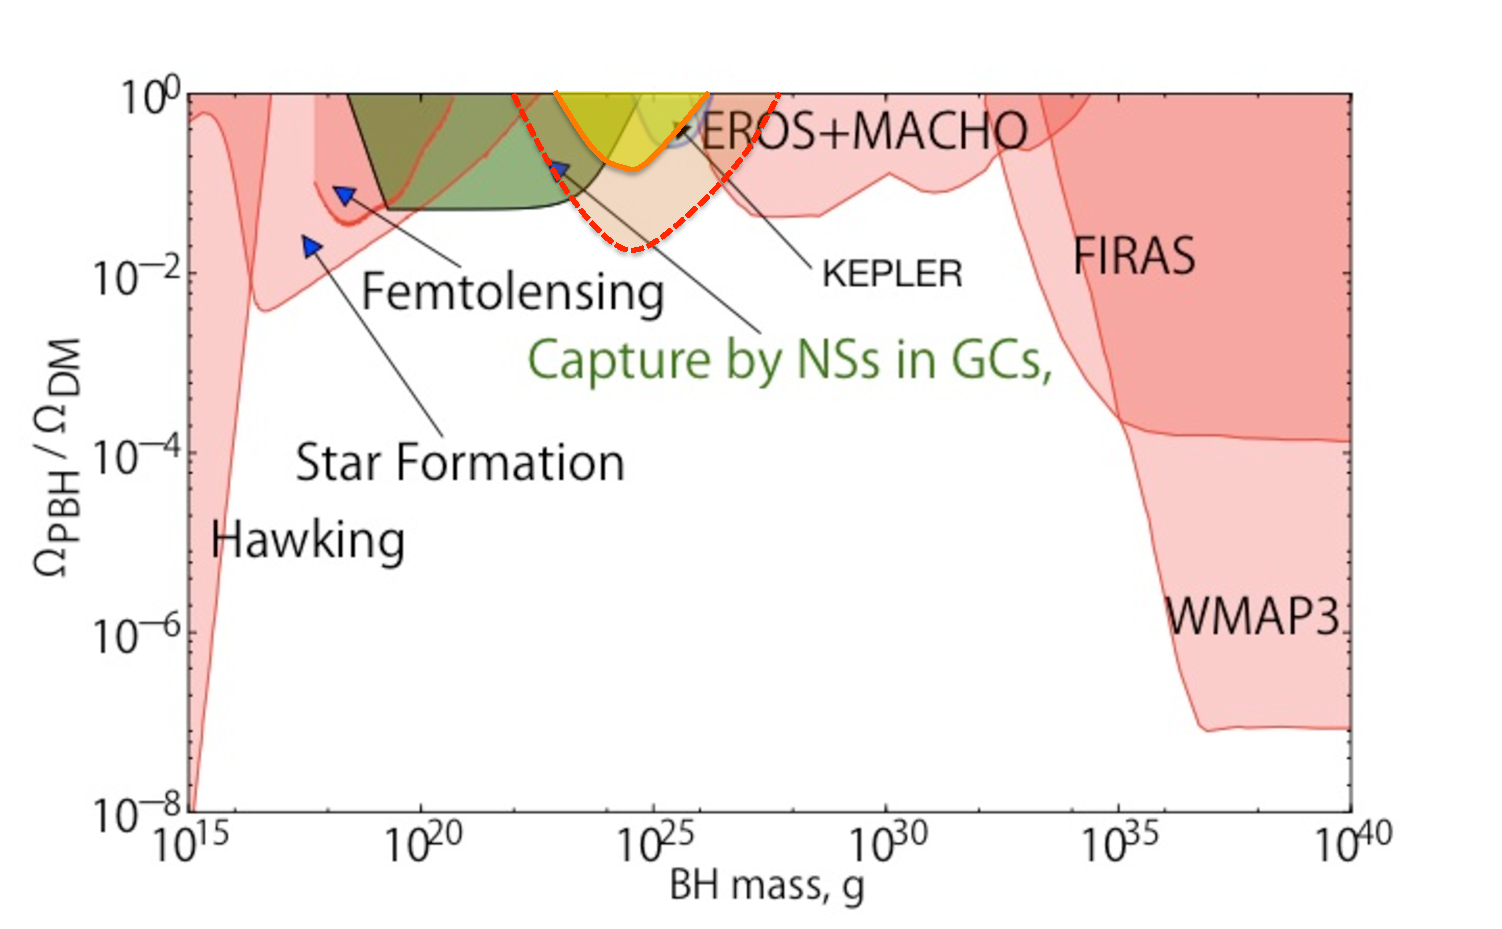
\includegraphics[width=0.6\textwidth]{pic/s14b_fig2-eps-converted-to.pdf}
\caption{\small{Summary of upper bound on the abundance of PBH, as its contribution to dark matter, in comparison with other constraints \citep{Capelaetal:13}. The orange line is the upper limit obtained from this thesis work using the 4 patch fields as used in Fig.~\ref{fig:dist}. The red dashed line is the constraint if using all the data of M31 (very preliminary) and assuming no detection of PBH microlensing. }}
\label{fig:pbhconst}
\end{figure*}


%\subsection{Interpretation}

\section{SUMMARY AND CONCLUSION}
\label{sec:dis2}
In this work 
we discussed our tests of nature of dark matter on star scales, and 
searched dark matter candidate so-called primordial black hole (PBH). 
We make use of microlensing effect for the search 
which is expected when PBH 
comes in the line of sight of background stars. 
Microlensing effect is rare event; only one in million stars can happen. 
Thus we used the Hyper Suprime-Cam (HSC) images of Andromeda Galaxy (M31) 
on stars in M31 to gather large number of stars and achieve higher event rate.  
The PBH is one of viable candidates for dark matter, and 
we performed tests to establish a way to constrain 
the abundance of PBHs of mass scales, $10^{-9}$-$10^{-7}M_\odot$, 
with the dense-cadence imaging data from wide-field camera.
One large problem is that 
default analysis mode of HSC-pipe software could not reduce the images with large number of stars; 
which caused troubles as in background subtraction, star catalog construction, 
image difference, and event detection. 
Therefore we managed to establish 
the reduction method as described in \S~\ref{sec:obs2} and \S~\ref{sec:res2}, to extract transient candidates from the images. 

From the reduced images we performed two kinds of analysis: 
transient study and microlensing implication. 
As for transient study we succeeded to extract as much as $\sim11,000$ transient candidates. 
We draw light curves for all the events and classified them 
by peak characteristics, $g$-$r$ color and magnitude. 
These characteristics help us figure out unique candidates  
as well as noise properties. 
The summary of candidate characteristics is provided 
in \S~\ref{sec:res2} and Appendix~\ref{sec:noncelestial} and \ref{sec:unieques}. 
We also started the second analysis; estimating microlensing properties and implication expected from our data.
Currently we could not find any microlensing candidates from the data 
by the fitting of theoretical microlensing light curve. 
Thus we started to estimate the upper limit of mass fraction of PBH to the total dark matter abundance implicated from our data. 
As our data covers large field of view, we need to take into account field-dependent properties 
such as star number counts and extinction. 
Therefore we divided the field of view into $10\times10$ sub-regions.  
In the first step we carefully looked into one single 
patch targeting region (patch=2,6) to reveal the position dependence, 
somehow succeeded to estimate the star number counts in the field.   
Our method constructed for one patch can be basically applied for wider field survey 
simply by considering position dependence and repeating the analysis. 
Also we make sure that our observation achieves 
strongest constraint on the mass fraction by simplified analysis. 

This project is still ongoing, and we might need further investigation of microlensing property. 
Especially disk and bulge region we might need further correction for  
estimating the magnitude or number counts of stars, 
because peak counts might not work for these regions. 
Also for microlensing event from PBHs in M31 halo region, 
we need to estimate the event rate more carefully by taking into account 
so-called finite-source effects or limb-darkening effect, 
which might greatly affect event time-scale estimation \citep[see][for the detail]{Riffeseretal:08}. 


The development achieved in our study can be applied to 
to future new time-space astronomy; aiming at faint, short-timescale events by 
wide-field or short-cadence survey. 
Currently several wide-field deep transient surveys are ongoing or planned not only by HSC, but also by 
the Palomar Transient Factory (PTF)\footnote{http://www.ptf.caltech.edu/iptf} and 
the Large Synoptic Survey Telescope (LSST)\footnote{http://www.lsst.org}. 
As for transient candidates, we can establish clear criteria 
to categorize the events like flares and binary stars including noise characteristics.  
Since our observation presents unique properties of faint, short-timescale variable candidates  
that has never been searched before, 
it would be helpful to characterize the time-dependent behavior of events 
in the future short cadence survey; 
as for microlensing study, event criteria can work as reference to 
remove contamination from microlensing candidates, for example. 

%%%%%%%%%%%%%%%%%%%%%%%%%%%%%%%%%%%%%%%%%%%%%%%%%%%%%%%%%%%%%%%%%%%%%%%%%%
% ACKNOWLEDGMENTS
%%%%%%%%%%%%%%%%%%%%%%%%%%%%%%%%%%%%%%%%%%%%%%%%%%%%%%%%%%%%%%%%%%%%%%%%%%
\section*{Acknowledgments}

MT was supported by World Premier International Research Center
Initiative (WPI Initiative), MEXT, Japan, by the FIRST program ``Subaru
Measurements of Images and Redshifts (SuMIRe)'', CSTP, Japan. MT was supported 
by Grant-in-Aid for Scientific Research from the JSPS Promotion of Science
(No.~23340061 and 26610058). 

\bibliographystyle{apj}
\bibliography{refs}


\end{document}
